\addcontentsline{toc}{chapter}{Matthew}
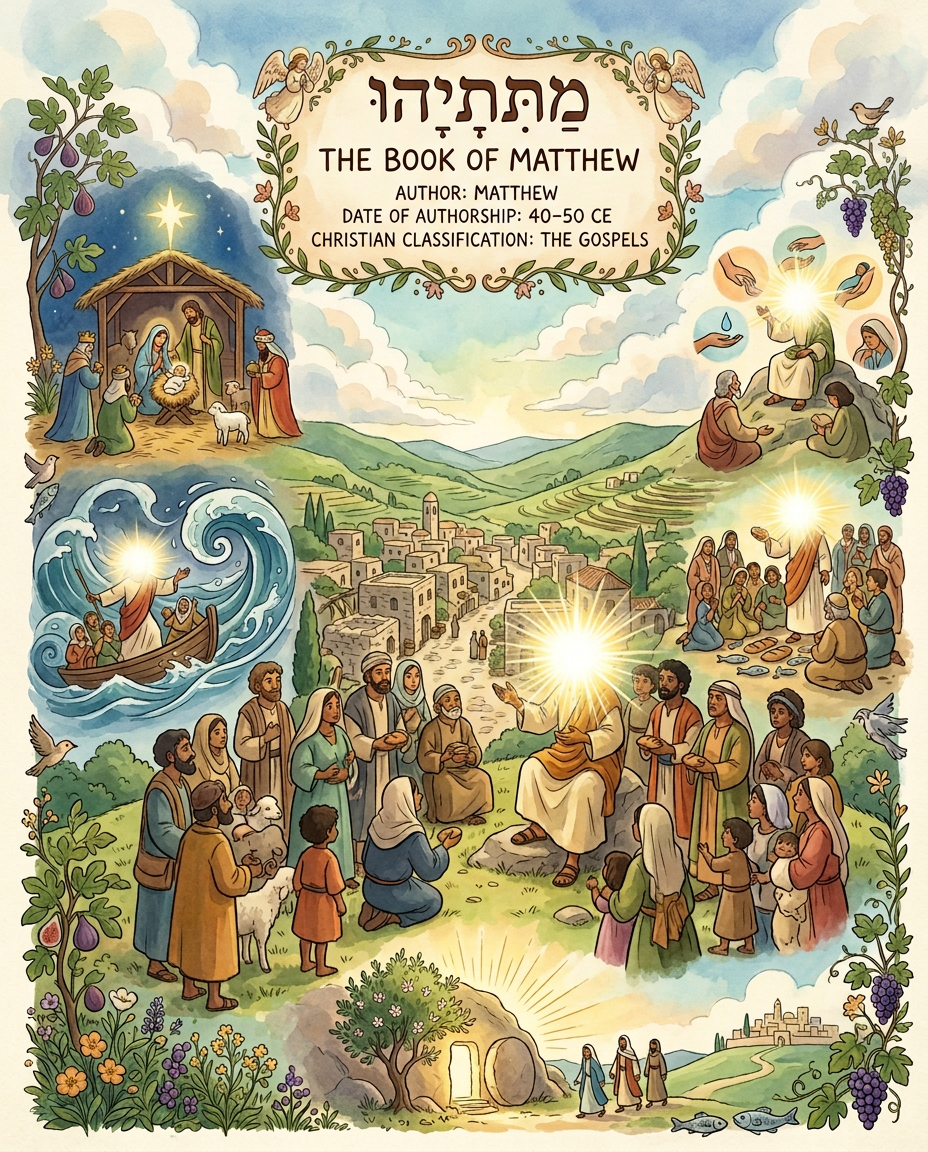
\includepdf[pages=1, fitpaper=false, width=\paperwidth, height=\paperheight, , keepaspectratio=false]{images/divider2/matthew2.png}
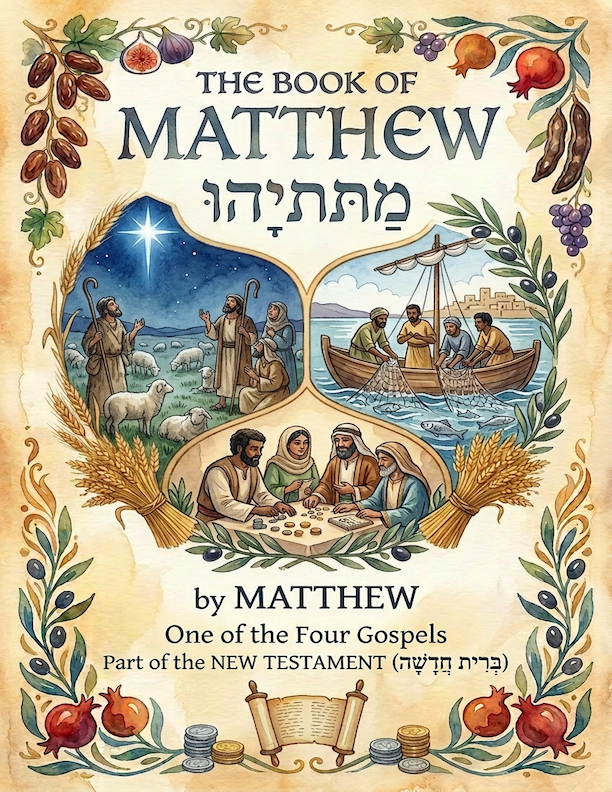
\includepdf[pages=1, fitpaper=false, width=\paperwidth, height=\paperheight, , keepaspectratio=false]{images/divider1/matthew.png}

\includepdf[pages=1, fitpaper=false, width=\paperwidth, height=\paperheight, , keepaspectratio=false]{images/8.5x11-Dot-Grid.png}

\includepdf[pages=1, fitpaper=false, width=\paperwidth, height=\paperheight, , keepaspectratio=false]{images/8.5x11-Dot-Grid.png}
\mybook{Matthew}
\vspace{-1.36in}


\mychapter{} \myverse*{}A record of the genealogy of Yeshua the Messiah,\footnote{1:1 Messiah (Hebrew) and Christ (Greek) both mean “Anointed One”} the son of David, the son
of Abraham.

\myverse{}Abraham became the father of Isaac. Isaac became the father of
Jacob. Jacob became the father of Judah and his brothers.
\myverse{}Judah became the father of Perez and Zerah by Tamar. Perez became the father
of Hezron. Hezron became the father of Ram.
\myverse{}Ram became the father of Amminadab. Amminadab became the father of Nahshon.
Nahshon became the father of Salmon.
\myverse{}Salmon became the father of Boaz by Rahab. Boaz became the father of Obed by
Ruth. Obed became the father of Jesse.
\myverse{}Jesse became the father of King David. David the king\footnote{1:6 NU omits “the king”.} became the father of Solomon by her who had been Uriah’s wife.
\myverse{}Solomon became the father of Rehoboam. Rehoboam became the father of Abijah.
Abijah became the father of Asa.
\myverse{}Asa became the father of Jehoshaphat. Jehoshaphat became the father of Joram.
Joram became the father of Uzziah.
\myverse{}Uzziah became the father of Jotham. Jotham became the father of Ahaz. Ahaz became
the father of Hezekiah.
\myverse{}Hezekiah became the father of Manasseh. Manasseh became the father of Amon.
Amon became the father of Josiah.
\myverse{}Josiah became the father of Jechoniah and his brothers at the time of the
exile to Babylon.

\myverse{}After the exile to Babylon, Jechoniah became the father of Shealtiel.
Shealtiel became the father of Zerubbabel.
\myverse{}Zerubbabel became the father of Abiud. Abiud became the father of Eliakim.
Eliakim became the father of Azor.
\myverse{}Azor became the father of Zadok. Zadok became the father of Achim. Achim became
the father of Eliud.
\myverse{}Eliud became the father of Eleazar. Eleazar became the father of Matthan.
Matthan became the father of Jacob.
\myverse{}Jacob became the father of Joseph, the husband of Miriam, from whom was born
Yeshua,\footnote{1:16 “Yeshua” means “Salvation”.} who is called Messiah.

\myverse{}So all the generations from Abraham to David are fourteen generations;
from David to the exile to Babylon fourteen generations; and from the carrying away to Babylon to the
Messiah, fourteen generations.

\myverse{}Now the birth of Yeshua the Messiah was like this: After his
mother, Miriam, was engaged to Joseph, before they came together, she was found pregnant by the Holy Spirit.
\myverse{}Joseph, her husband, being a righteous man, and not willing to make her a
public example, intended to put her away secretly.
\myverse{}But when he thought about these things, behold,\footnote{1:20 “Behold”, from “ἰδοὺ”, means look at, take notice, observe, see, or gaze at. It is often used
	as an interjection.} an angel of the Lord appeared to him in a dream, saying, “Joseph, son of
David, don’t be afraid to take to yourself Miriam as your wife, for that which is conceived in her is
of the Holy Spirit.
\myverse{}She shall give birth to a son. You shall name him Yeshua,\footnote{1:21 “Yeshua” means “Salvation”.} for it is he who shall save his people from their sins.”

\myverse{}Now all this has happened that it might be fulfilled which was
spoken by the Lord through the prophet, saying,

\myverse{}“Behold, the virgin shall be with child,

and shall give birth to a son.

They shall call his name Immanuel,”

which is, being interpreted, “God with us.”\footnote{1:23 Isaiah 7:14}

\myverse{}Joseph arose from his sleep, and did as the angel of the Lord
commanded him, and took his wife to himself;
\myverse{}and didn’t know her sexually until she had given birth to her firstborn son.
He named him Yeshua.


% Matthew 2
\mychapter{} \myverse*{}Now when Yeshua was born in Bethlehem of Judea in the days of King
Herod, behold, wise men\footnote{2:1 The word for “wise men” (magoi) can also mean teachers, scientists, physicians, astrologers,
	seers, interpreters of dreams, or sorcerers.} from the east came to Jerusalem, saying,
\myverse{}“Where is he who is born King of the Jews? For we saw his star in the east,
and have come to worship him.”
\myverse{}When King Herod heard it, he was troubled, and all Jerusalem with him.
\myverse{}Gathering together all the chief priests and scribes of the people, he asked
them where the Messiah would be born.
\myverse{}They said to him, “In Bethlehem of Judea, for this is written through the prophet,

\myverse{}‘You Bethlehem, land of Judah,

are in no way least among the princes of Judah;

for out of you shall come a governor

who shall shepherd my people, Israel.’ ”\footnote{2:6 Micah 5:2}

\myverse{}Then Herod secretly called the wise men, and learned from them
exactly what time the star appeared.
\myverse{}He sent them to Bethlehem, and said, “Go and search diligently for the young
child. When you have found him, bring me word, so that I also may come and worship him.”

\myverse{}They, having heard the king, went their way; and behold, the star,
which they saw in the east, went before them until it came and stood over where the young child was.
\myverse{}When they saw the star, they rejoiced with exceedingly great joy.
\myverse{}They came into the house and saw the young child with Miriam, his mother,
and they fell down and worshiped him. Opening their treasures, they offered to him gifts: gold, frankincense,
and myrrh.
\myverse{}Being warned in a dream not to return to Herod, they went back to their own
country another way.

\myverse{}Now when they had departed, behold, an angel of the Lord appeared
to Joseph in a dream, saying, “Arise and take the young child and his mother, and flee into Egypt, and
stay there until I tell you, for Herod will seek the young child to destroy him.”

\myverse{}He arose and took the young child and his mother by night and
departed into Egypt,
\myverse{}and was there until the death of Herod, that it might be fulfilled which was
spoken by the Lord through the prophet, saying, “Out of Egypt I called my son.”\footnote{2:15 Hosea 11:1}

\myverse{}Then Herod, when he saw that he was mocked by the wise men, was
exceedingly angry, and sent out and killed all the male children who were in Bethlehem and in all the
surrounding countryside, from two years old and under, according to the exact time which he had learned
from the wise men.
\myverse{}Then that which was spoken by Jeremiah the prophet was fulfilled, saying,

\myverse{}“A voice was heard in Ramah,

lamentation, weeping and great mourning,

Rachel weeping for her children;

she wouldn’t be comforted,

because they are no more.”\footnote{2:18 Jeremiah 31:15}

\myverse{}But when Herod was dead, behold, an angel of the Lord appeared
in a dream to Joseph in Egypt, saying,
\myverse{}“Arise and take the young child and his mother, and go into Eretz-Israel,
for those who sought the young child’s life are dead.”

\myverse{}He arose and took the young child and his mother, and came into
Eretz-Israel.
\myverse{}But when he heard that Archelaus was reigning over Judea in the place of his
father, Herod, he was afraid to go there. Being warned in a dream, he withdrew into the region of Galilee,
\myverse{}and came and lived in a city called Nazareth; that it might be fulfilled which
was spoken through the prophets that he will be called a Nazarene.


% MATTHEW 3
\mychapter{} \myverse*{}In those days, Yochanan the Immerser came, proclaiming in the wilderness
of Judea, saying,
\myverse{}“Repent, for the Kingdom of Heaven is at hand!”
\myverse{}For this is he who was spoken of by Isaiah the prophet, saying,

“The voice of one crying in the wilderness,

make the way of the Lord ready!

Make his paths straight!”\footnote{3:3 Isaiah 40:3}

\myverse{}Now Yochanan himself wore clothing made of camel’s hair with a
leather belt around his waist. His food was locusts and wild honey.
\myverse{}Then people from Jerusalem, all of Judea, and all the region around the Jordan
went out to him.
\myverse{}They were immersed by him in the Jordan, confessing their sins.

\myverse{}But when he saw many of the Pharisees and Sadducees coming for
his immersion, he said to them, “You offspring of vipers, who warned you to flee from the wrath to come?
\myverse{}Therefore produce fruit worthy of repentance!
\myverse{}Don’t think to yourselves, ‘We have Abraham for our father,’ for I tell you
that God is able to raise up children to Abraham from these stones.
\myverse{}Even now the ax lies at the root of the trees. Therefore every tree that doesn’t
produce good fruit is cut down, and cast into the fire.

\myverse{}“I indeed immerse you in water for repentance, but he who comes
after me is mightier than I, whose sandals I am not worthy to carry. He will immerse you in the Holy Spirit.\footnote{3:11 TR and NU add “and with fire”
}
\myverse{}His winnowing fork is in his hand, and he will thoroughly cleanse his threshing
floor. He will gather his wheat into the barn, but the chaff he will burn up with unquenchable fire.”

\myverse{}Then Yeshua came from Galilee to the Jordan\footnote{3:13 i.e., the Jordan River} to Yochanan, to be immersed by him.
\myverse{}But Yochanan would have hindered him, saying, “I need to be immersed by you,
and you come to me?”

\myverse{}But Yeshua, answering, said to him,
\textcolor{crimson}{“Allow it now, for this is the fitting way for us to fulfill all righteousness.”} Then he allowed
him.

\myverse{}Yeshua, when he was immersed, went up directly from the water:
and behold, the heavens were opened to him. He saw the Spirit of God descending as a dove, and coming
on him.
\myverse{}Behold, a voice out of the heavens said, “This is my beloved Son, with whom
I am well pleased.”


% MATTHEW 4
\mychapter{} \myverse*{}Then Yeshua was led up by the Spirit into the wilderness to be
tempted by the devil.
\myverse{}When he had fasted forty days and forty nights, he was hungry afterward.
\myverse{}The tempter came and said to him, “If you are the Son of God, command that these
stones become bread.”

\myverse{}But he answered,
\textcolor{crimson}{“It is written, ‘Man shall not live by bread alone, but by every word that proceeds out of God’s mouth.’ ”}\footnote{4:4 Deuteronomy 8:3}

\myverse{}Then the devil took him into the holy city. He set him on the pinnacle
of the temple,
\myverse{}and said to him, “If you are the Son of God, throw yourself down, for it is
written,

‘He will command his angels concerning you,’ and,

‘On their hands they will bear you up,

so that you don’t dash your foot against a stone.’ ”\footnote{4:6 Psalms 91:11-12
}

\myverse{}Yeshua said to him,
\textcolor{crimson}{“Again, it is written, ‘You shall not test the Lord, your God.’ ”}\footnote{4:7 Deuteronomy 6:16}

\myverse{}Again, the devil took him to an exceedingly high mountain, and
showed him all the kingdoms of the world and their glory.
\myverse{}He said to him, “I will give you all of these things, if you will fall down
and worship me.”

\myverse{}Then Yeshua said to him,
\textcolor{crimson}{“Get behind me,}\footnote{4:10 TR and NU read “Go away” instead of “Get behind me”}
\textcolor{crimson}{Satan! For it is written, ‘You shall worship the Lord your God, and you shall serve him only.’ ”}
\footnote{4:10 Deuteronomy 6:13}

\myverse{}Then the devil left him, and behold, angels came and served him.

\myverse{}Now when Yeshua heard that Yochanan was delivered up, he withdrew
into Galilee.
\myverse{}Leaving Nazareth, he came and lived in Capernaum, which is by the sea, in
the region of Zebulun and Naphtali,
\myverse{}that it might be fulfilled which was spoken through Isaiah the prophet, saying,

\myverse{}“The land of Zebulun and the land of Naphtali,

toward the sea, beyond the Jordan,

Galilee of the Gentiles,

\myverse{}the people who sat in darkness saw a great light;

to those who sat in the region and shadow of death,

to them light has dawned.”\footnote{4:16 Isaiah 9:1-2}

\myverse{}From that time, Yeshua began to proclaim, and to say,
\textcolor{crimson}{“Repent! For the Kingdom of Heaven is at hand.”}

\myverse{}Walking by the sea of Galilee, he\footnote{4:18 TR reads “Yeshua” instead of “he”
} saw two brothers: Simon, who is called Peter, and Andrew, his brother, casting a net into the
sea; for they were fishermen.
\myverse{}He said to them,
\textcolor{crimson}{“Come after me, and I will make you fishers for men.”}

\myverse{}They immediately left their nets and followed him.
\myverse{}Going on from there, he saw two other brothers, Jacob the son of Zebedee,
and Yochanan his brother, in the boat with Zebedee their father, mending their nets. He called them.
\myverse{}They immediately left the boat and their father, and followed him.

\myverse{}Yeshua went about in all Galilee, teaching in their synagogues,
proclaiming the Good News of the Kingdom, and healing every disease and every sickness among the people.
\myverse{}The report about him went out into all Syria. They brought to him all who
were sick, afflicted with various diseases and torments, possessed with demons, epileptics, and paralytics;
and he healed them.
\myverse{}Great multitudes from Galilee, Decapolis, Jerusalem, Judea, and from beyond
the Jordan followed him.


% MATTHEW 5
\mychapter{} \myverse*{}Seeing the multitudes, he went up onto the mountain. When he had
sat down, his disciples came to him.
\myverse{}He opened his mouth and taught them, saying,

\myverse{}\textcolor{crimson}{“Blessed are the poor in spirit,}

\textcolor{crimson}{for theirs is the Kingdom of Heaven.}\footnote{5:3 Isaiah 57:15;
	66:2}

\myverse{}\textcolor{crimson}{Blessed are those who mourn,}

\textcolor{crimson}{for they shall be comforted.}\footnote{5:4 Isaiah 61:2;
	66:10,13}

\myverse{}\textcolor{crimson}{Blessed are the gentle,}

\textcolor{crimson}{for they shall inherit the earth.}\footnote{5:5 or, land.}\footnote{5:5 Psalms 37:11}

\myverse{}\textcolor{crimson}{Blessed are those who hunger and thirst for righteousness,
}

\textcolor{crimson}{for they shall be filled.}

\myverse{}\textcolor{crimson}{Blessed are the merciful,}

\textcolor{crimson}{for they shall obtain mercy.}

\myverse{}\textcolor{crimson}{Blessed are the pure in heart,}

\textcolor{crimson}{for they shall see God.}

\myverse{}\textcolor{crimson}{Blessed are the peacemakers,}

\textcolor{crimson}{for they shall be called children of God.}

\myverse{}\textcolor{crimson}{Blessed are those who have been persecuted for righteousness’
	sake,
}

\textcolor{crimson}{for theirs is the Kingdom of Heaven.}

\myverse{}\textcolor{crimson}{“Blessed are you when people reproach you, persecute you,
	and say all kinds of evil against you falsely, for my sake.
}
\myverse{}\textcolor{crimson}{Rejoice, and be exceedingly glad, for great is your reward in heaven.
	For that is how they persecuted the prophets who were before you.
}

\myverse{}\textcolor{crimson}{“You are the salt of the earth, but if the salt has lost
	its flavor, with what will it be salted? It is then good for nothing, but to be cast out and trodden under
	the feet of men.
}

\myverse{}\textcolor{crimson}{“You are the light of the world. A city located on a hill
	can’t be hidden.
}
\myverse{}\textcolor{crimson}{Neither do you light a lamp and put it under a measuring basket, but on
	a stand; and it shines to all who are in the house.
}
\myverse{}\textcolor{crimson}{Even so, let your light shine before men, that they may see your good
	works and glorify your Father who is in heaven.}

\myverse{}\textcolor{crimson}{“Don’t think that I came to destroy the Torah or the Prophets.
	I didn’t come to destroy, but to fulfill.
}
\myverse{}\textcolor{crimson}{For most certainly, I tell you, until heaven and earth pass away, not
	even one smallest letter}\footnote{5:18 literally, iota}
\textcolor{crimson}{or one tiny pen stroke}\footnote{5:18 or, serif}
\textcolor{crimson}{shall in any way pass away from the Torah, until all things are accomplished.
}
\myverse{}\textcolor{crimson}{Therefore, whoever shall break one of these least commandments and teach
	others to do so, shall be called least in the Kingdom of Heaven; but whoever shall do and teach them shall
	be called great in the Kingdom of Heaven.
}
\myverse{}\textcolor{crimson}{For I tell you that unless your righteousness exceeds that of the scribes
	and Pharisees, there is no way you will enter into the Kingdom of Heaven.}

\myverse{}\textcolor{crimson}{“You have heard that it was said to the ancient ones, ‘You
	shall not murder;’}\footnote{5:21 Exodus 20:13}
\textcolor{crimson}{and ‘Whoever murders will be in danger of the judgment.’
}
\myverse{}\textcolor{crimson}{But I tell you that everyone who is angry with his brother without a cause
}\footnote{5:22 NU omits “without a cause”.}
\textcolor{crimson}{will be in danger of the judgment. Whoever says to his brother, ‘You good-for-nothing!’
}\footnote{5:22 “You good-for-nothing” is an Aramaic insult, related to the word for “empty” and conveying the
	idea of empty-headedness.}
\textcolor{crimson}{will be in danger of the council. Whoever says, ‘You fool!’ will be in danger of the fire of Gehinnom.}\footnote{5:22 or, Hell}

\myverse{}\textcolor{crimson}{“If therefore you are offering your gift at the altar, and
	there remember that your brother has anything against you,
}
\myverse{}\textcolor{crimson}{leave your gift there before the altar, and go your way. First be reconciled
	to your brother, and then come and offer your gift.
}
\myverse{}\textcolor{crimson}{Agree with your adversary quickly while you are with him on the way; lest
	perhaps the prosecutor deliver you to the judge, and the judge deliver you to the officer, and you be
	cast into prison.
}
\myverse{}\textcolor{crimson}{Most certainly I tell you, you shall by no means get out of there until
	you have paid the last penny.}\footnote{5:26 literally, kodrantes. A kodrantes was a small copper coin worth about 2 lepta (widow’s mites)—not
	enough to buy very much of anything.}

\myverse{}\textcolor{crimson}{“You have heard that it was said,
}\footnote{5:27 TR adds “to the ancients”.}
\textcolor{crimson}{‘You shall not commit adultery;’}\footnote{5:27 Exodus 20:14}
\myverse{}\textcolor{crimson}{but I tell you that everyone who gazes at a woman to lust after her has
	committed adultery with her already in his heart.
}
\myverse{}\textcolor{crimson}{If your right eye causes you to stumble, pluck it out and throw it away
	from you. For it is more profitable for you that one of your members should perish than for your whole
	body to be cast into Gehinnom.}\footnote{5:29 or, Hell}
\myverse{}\textcolor{crimson}{If your right hand causes you to stumble, cut it off, and throw it away
	from you. For it is more profitable for you that one of your members should perish, than for your whole
	body to be cast into Gehinnom.}\footnote{5:30 or, Hell}

\myverse{}\textcolor{crimson}{“It was also said, ‘Whoever shall put away his wife, let
	him give her a writing of divorce,’}\footnote{5:31 Deuteronomy 24:1}
\myverse{}\textcolor{crimson}{but I tell you that whoever puts away his wife, except for the cause of
	sexual immorality, makes her an adulteress; and whoever marries her when she is put away commits adultery.}

\myverse{}\textcolor{crimson}{“Again you have heard that it was said to the ancient ones,
	‘You shall not make false vows, but shall perform to the Lord your vows,’}\footnote{5:33 Numbers 30:2;
	Deuteronomy 23:21;
	Ecclesiastes 5:4}
\myverse{}\textcolor{crimson}{but I tell you, don’t swear at all: neither by heaven, for it is the throne
	of God;
}
\myverse{}\textcolor{crimson}{nor by the earth, for it is the footstool of his feet; nor by Jerusalem,
	for it is the city of the great King.
}
\myverse{}\textcolor{crimson}{Neither shall you swear by your head, for you can’t make one hair white
	or black.
}
\myverse{}\textcolor{crimson}{But let your ‘Yes’ be ‘Yes’ and your ‘No’ be ‘No.’ Whatever is more than
	these is of the evil one.}

\myverse{}\textcolor{crimson}{“You have heard that it was said, ‘An eye for an eye, and
	a tooth for a tooth.’}\footnote{5:38 Exodus 21:24;
	Leviticus 24:20;
	Deuteronomy 19:21}
\myverse{}\textcolor{crimson}{But I tell you, don’t resist him who is evil; but whoever strikes you
	on your right cheek, turn to him the other also.
}
\myverse{}\textcolor{crimson}{If anyone sues you to take away your coat, let him have your cloak also.
}
\myverse{}\textcolor{crimson}{Whoever compels you to go one mile, go with him two.
}
\myverse{}\textcolor{crimson}{Give to him who asks you, and don’t turn away him who desires to borrow
	from you.}

\myverse{}\textcolor{crimson}{“You have heard that it was said, ‘You shall love your neighbor
}\footnote{5:43 Leviticus 19:18}
\textcolor{crimson}{and hate your enemy.’}\footnote{5:43 not in the Bible, but see Qumran Manual of Discipline Ix, 21-26}
\myverse{}\textcolor{crimson}{But I tell you, love your enemies, bless those who curse you, do good
	to those who hate you, and pray for those who mistreat you and persecute you,
}
\myverse{}\textcolor{crimson}{that you may be children of your Father who is in heaven. For he makes
	his sun to rise on the evil and the good, and sends rain on the just and the unjust.
}
\myverse{}\textcolor{crimson}{For if you love those who love you, what reward do you have? Don’t even
	the tax collectors do the same?
}
\myverse{}\textcolor{crimson}{If you only greet your friends, what more do you do than others? Don’t
	even the tax collectors}\footnote{5:47 NU reads “Gentiles” instead of “tax collectors”.}
\textcolor{crimson}{do the same?
}
\myverse{}\textcolor{crimson}{Therefore you shall be perfect, just as your Father in heaven is perfect.}


% MATTEHEW 6
\mychapter{} \myverse*{}\textcolor{crimson}{“Be careful that you don’t do your charitable giving}\footnote{6:1 NU reads “acts of righteousness” instead of “charitable giving”}
\textcolor{crimson}{before men, to be seen by them, or else you have no reward from your Father who is in heaven.
}
\myverse{}\textcolor{crimson}{Therefore, when you do merciful deeds, don’t sound a shofar before yourself,
	as the hypocrites do in the synagogues and in the streets, that they may get glory from men. Most certainly
	I tell you, they have received their reward.
}
\myverse{}\textcolor{crimson}{But when you do merciful deeds, don’t let your left hand know what your
	right hand does,
}
\myverse{}\textcolor{crimson}{so that your merciful deeds may be in secret, then your Father who sees
	in secret will reward you openly.}

\myverse{}\textcolor{crimson}{“When you pray, you shall not be as the hypocrites, for they
	love to stand and pray in the synagogues and in the corners of the streets, that they may be seen by men.
	Most certainly, I tell you, they have received their reward.
}
\myverse{}\textcolor{crimson}{But you, when you pray, enter into your inner room, and having shut your
	door, pray to your Father who is in secret; and your Father who sees in secret will reward you openly.
}
\myverse{}\textcolor{crimson}{In praying, don’t use vain repetitions as the Gentiles do; for they think
	that they will be heard for their much speaking.
}
\myverse{}\textcolor{crimson}{Therefore don’t be like them, for your Father knows what things you need
	before you ask him.
}
\myverse{}\textcolor{crimson}{Pray like this:
}

\textcolor{crimson}{“ ‘Our Father in heaven, may your name be kept holy.
}

\myverse{}\textcolor{crimson}{Let your Kingdom come.
}

\textcolor{crimson}{Let your will be done on earth as it is in heaven.
}

\myverse{}\textcolor{crimson}{Give us today our daily bread.
}

\myverse{}\textcolor{crimson}{Forgive us our debts,}

\textcolor{crimson}{as we also forgive our debtors.
}

\myverse{}\textcolor{crimson}{Bring us not into temptation,}

\textcolor{crimson}{but deliver us from the evil one.}

\textcolor{crimson}{For yours is the Kingdom, the power, and the glory forever. Amen.’}\footnote{6:13 NU omits “For yours is the Kingdom, the power, and the glory forever. Amen.”}

\myverse{}\textcolor{crimson}{“For if you forgive men their trespasses, your heavenly Father
	will also forgive you.
}
\myverse{}\textcolor{crimson}{But if you don’t forgive men their trespasses, neither will your Father
	forgive your trespasses.}

\myverse{}\textcolor{crimson}{“Moreover when you fast, don’t be like the hypocrites, with
	sad faces. For they disfigure their faces that they may be seen by men to be fasting. Most certainly I
	tell you, they have received their reward.
}
\myverse{}\textcolor{crimson}{But you, when you fast, anoint your head and wash your face,
}
\myverse{}\textcolor{crimson}{so that you are not seen by men to be fasting, but by your Father who
	is in secret; and your Father, who sees in secret, will reward you.
}

\myverse{}\textcolor{crimson}{“Don’t lay up treasures for yourselves on the earth, where
	moth and rust consume, and where thieves break through and steal;
}
\myverse{}\textcolor{crimson}{but lay up for yourselves treasures in heaven, where neither moth nor
	rust consume, and where thieves don’t break through and steal;
}
\myverse{}\textcolor{crimson}{for where your treasure is, there your heart will be also.
}

\myverse{}\textcolor{crimson}{“The lamp of the body is the eye. If therefore your eye is
	sound, your whole body will be full of light.
}
\myverse{}\textcolor{crimson}{But if your eye is evil, your whole body will be full of darkness. If
	therefore the light that is in you is darkness, how great is the darkness!
}

\myverse{}\textcolor{crimson}{“No one can serve two masters, for either he will hate the
	one and love the other, or else he will be devoted to one and despise the other. You can’t serve both
	God and Mammon.
}
\myverse{}\textcolor{crimson}{Therefore I tell you, don’t be anxious for your life: what you will eat,
	or what you will drink; nor yet for your body, what you will wear. Isn’t life more than food, and the
	body more than clothing?
}
\myverse{}\textcolor{crimson}{See the birds of the sky, that they don’t sow, neither do they reap, nor
	gather into barns. Your heavenly Father feeds them. Aren’t you of much more value than they?}

\myverse{}\textcolor{crimson}{“Which of you by being anxious, can add one moment}\footnote{6:27 literally, cubit}
\textcolor{crimson}{to his lifespan?
}
\myverse{}\textcolor{crimson}{Why are you anxious about clothing? Consider the lilies of the field,
	how they grow. They don’t toil, neither do they spin,
}
\myverse{}\textcolor{crimson}{yet I tell you that even Solomon in all his glory was not dressed like
	one of these.
}
\myverse{}\textcolor{crimson}{But if God so clothes the grass of the field, which today exists and tomorrow
	is thrown into the oven, won’t he much more clothe you, you of little faith?}

\myverse{}\textcolor{crimson}{“Therefore don’t be anxious, saying, ‘What will we eat?’,
	‘What will we drink?’ or, ‘With what will we be clothed?’
}
\myverse{}\textcolor{crimson}{For the Gentiles seek after all these things; for your heavenly Father
	knows that you need all these things.
}
\myverse{}\textcolor{crimson}{But seek first God’s Kingdom and his righteousness; and all these things
	will be given to you as well.
}
\myverse{}\textcolor{crimson}{Therefore don’t be anxious for tomorrow, for tomorrow will be anxious
	for itself. Each day’s own evil is sufficient.}


% MATTHEW 7
\mychapter{} \myverse*{}\textcolor{crimson}{“Don’t judge, so that you won’t be judged.
}
\myverse{}\textcolor{crimson}{For with whatever judgment you judge, you will be judged; and with whatever
	measure you measure, it will be measured to you.
}
\myverse{}\textcolor{crimson}{Why do you see the speck that is in your brother’s eye, but don’t consider
	the beam that is in your own eye?
}
\myverse{}\textcolor{crimson}{Or how will you tell your brother, ‘Let me remove the speck from your eye,’
	and behold, the beam is in your own eye?
}
\myverse{}\textcolor{crimson}{You hypocrite! First remove the beam out of your own eye, and then you can
	see clearly to remove the speck out of your brother’s eye.}

\myverse{}\textcolor{crimson}{“Don’t give that which is holy to the dogs, neither throw your
	pearls before the pigs, lest perhaps they trample them under their feet, and turn and tear you to pieces.}

\myverse{}\textcolor{crimson}{“Ask, and it will be given you. Seek, and you will find. Knock,
	and it will be opened for you.
}
\myverse{}\textcolor{crimson}{For everyone who asks receives. He who seeks finds. To him who knocks it
	will be opened.
}
\myverse{}\textcolor{crimson}{Or who is there among you who, if his son asks him for bread, will give
	him a stone?
}
\myverse{}\textcolor{crimson}{Or if he asks for a fish, who will give him a serpent?} \myverse{}\textcolor{crimson}{If you then, being evil, know how to give good gifts to your children,	how much more will your Father who is in heaven give good things to those who ask him!} \myverse{}\textcolor{crimson}{Therefore, whatever you desire for men to do to you, you shall also do to them; for this is the Torah and the Prophets.}

\myverse{}\textcolor{crimson}{“Enter in by the narrow gate; for the gate is wide and the
	way is broad that leads to destruction, and there are many who enter in by it.
}
\myverse{}\textcolor{crimson}{How}\footnote{7:14 TR reads “Because” instead of “How”}
\textcolor{crimson}{narrow is the gate and the way is restricted that leads to life! There are few who find it.}

\myverse{}\textcolor{crimson}{“Beware of false prophets, who come to you in sheep’s clothing,
	but inwardly are ravening wolves.
}
\myverse{}\textcolor{crimson}{By their fruits you will know them. Do you gather grapes from thorns or
	figs from thistles?
}
\myverse{}\textcolor{crimson}{Even so, every good tree produces good fruit, but the corrupt tree produces
	evil fruit.
}
\myverse{}\textcolor{crimson}{A good tree can’t produce evil fruit, neither can a corrupt tree produce
	good fruit.
}
\myverse{}\textcolor{crimson}{Every tree that doesn’t grow good fruit is cut down and thrown into the
	fire.
}
\myverse{}\textcolor{crimson}{Therefore by their fruits you will know them.
}

\myverse{}\textcolor{crimson}{“Not everyone who says to me, ‘Lord, Lord,’ will enter into
	the Kingdom of Heaven, but he who does the will of my Father who is in heaven.
}
\myverse{}\textcolor{crimson}{Many will tell me in that day, ‘Lord, Lord, didn’t we prophesy in your
	name, in your name cast out demons, and in your name do many mighty works?’
}
\myverse{}\textcolor{crimson}{Then I will tell them, ‘I never knew you. Depart from me, you who work
	iniquity.’}

\myverse{}\textcolor{crimson}{“Everyone therefore who hears these words of mine and does
	them, I will liken him to a wise man who built his house on the rock.
}
\myverse{}\textcolor{crimson}{The rain came down, the floods came, and the winds blew and beat on that
	house; and it didn’t fall, for it was founded on the rock.
}
\myverse{}\textcolor{crimson}{Everyone who hears these words of mine and doesn’t do them will be like
	a foolish man who built his house on the sand.
}
\myverse{}\textcolor{crimson}{The rain came down, the floods came, and the winds blew and beat on that
	house; and it fell—and its fall was great.”}

\myverse{}When Yeshua had finished saying these things, the multitudes
were astonished at his teaching,
\myverse{}for he taught them with authority, and not like the scribes.


% MATTHEW 8
\mychapter{} \myverse*{}When he came down from the mountain, great multitudes followed
him.
\myverse{}Behold, a leper came to him and worshiped him, saying, “Lord, if you want to,
you can make me clean.”

\myverse{}Yeshua stretched out his hand and touched him, saying,
\textcolor{crimson}{“I want to. Be made clean.”} Immediately his leprosy was cleansed.
\myverse{}Yeshua said to him,
\textcolor{crimson}{“See that you tell nobody; but go, show yourself to the priest, and offer the gift that Moses commanded,
	as a testimony to them.”}

\myverse{}When he came into Capernaum, a centurion came to him, asking him
for help,
\myverse{}saying, “Lord, my servant lies in the house paralyzed, grievously tormented.”

\myverse{}Yeshua said to him,
\textcolor{crimson}{“I will come and heal him.”}

\myverse{}The centurion answered, “Lord, I’m not worthy for you to come under
my roof. Just say the word, and my servant will be healed.
\myverse{}For I am also a man under authority, having under myself soldiers. I tell this
one, ‘Go,’ and he goes; and tell another, ‘Come,’ and he comes; and tell my servant, ‘Do this,’ and he
does it.”

\myverse{}When Yeshua heard it, he marveled and said to those who followed,
\textcolor{crimson}{“Most certainly I tell you, I haven’t found so great a faith, not even in Israel.
}
\myverse{}\textcolor{crimson}{I tell you that many will come from the east and the west, and will sit
	down with Abraham, Isaac, and Jacob in the Kingdom of Heaven,
}
\myverse{}\textcolor{crimson}{but the children of the Kingdom will be thrown out into the outer darkness.
	There will be weeping and gnashing of teeth.”}
\myverse{}Yeshua said to the centurion,
\textcolor{crimson}{“Go your way. Let it be done for you as you have believed.”} His servant was healed in that hour.

\myverse{}When Yeshua came into Peter’s house, he saw his wife’s mother
lying sick with a fever.
\myverse{}He touched her hand, and the fever left her. So she got up and served him.\footnote{8:15 TR reads “them” instead of “him”}
\myverse{}When evening came, they brought to him many possessed with demons. He cast
out the spirits with a word, and healed all who were sick,
\myverse{}that it might be fulfilled which was spoken through Isaiah the prophet, saying,
“He took our infirmities and bore our diseases.”\footnote{8:17 Isaiah 53:4
}

\myverse{}Now when Yeshua saw great multitudes around him, he gave the
order to depart to the other side.

\myverse{}A scribe came and said to him, “Rabbi, I will follow you wherever
you go.”

\myverse{}Yeshua said to him,
\textcolor{crimson}{“The foxes have holes and the birds of the sky have nests, but the Son of Man has nowhere to lay his
	head.”}

\myverse{}Another of his disciples said to him, “Lord, allow me first to
go and bury my father.”

\myverse{}But Yeshua said to him,
\textcolor{crimson}{“Follow me, and leave the dead to bury their own dead.”}

\myverse{}When he got into a boat, his disciples followed him.
\myverse{}Behold, a violent storm came up on the sea, so much that the boat was covered
with the waves; but he was asleep.
\myverse{}The disciples came to him and woke him up, saying, “Save us, Lord! We are
dying!”

\myverse{}He said to them,
\textcolor{crimson}{“Why are you fearful, O you of little faith?”
} Then he got up, rebuked the wind and the sea, and there was a great calm.

\myverse{}The men marveled, saying, “What kind of man is this, that even
the wind and the sea obey him?”

\myverse{}When he came to the other side, into the country of the Gergesenes,\footnote{8:28 NU reads “Gadarenes”} two people possessed by demons met him there, coming out of the
tombs, exceedingly fierce, so that nobody could pass that way.
\myverse{}Behold, they cried out, saying, “What do we have to do with you, Yeshua, Son
of God? Have you come here to torment us before the time?”
\myverse{}Now there was a herd of many pigs feeding far away from them.
\myverse{}The demons begged him, saying, “If you cast us out, permit us to go away into
the herd of pigs.”

\myverse{}He said to them,
\textcolor{crimson}{“Go!”}

They came out and went into the herd of pigs; and behold, the whole herd of pigs rushed down
the cliff into the sea and died in the water.
\myverse{}Those who fed them fled and went away into the city and told everything, including
what happened to those who were possessed with demons.
\myverse{}Behold, all the city came out to meet Yeshua. When they saw him, they begged
that he would depart from their borders.


% MATTHEW 9
\mychapter{} \myverse*{}He entered into a boat and crossed over, and came into his own
city.
\myverse{}Behold, they brought to him a man who was paralyzed, lying on a bed. Yeshua,
seeing their faith, said to the paralytic,
\textcolor{crimson}{“Son, cheer up! Your sins are forgiven you.”}

\myverse{}Behold, some of the scribes said to themselves, “This man blasphemes.”

\myverse{}Yeshua, knowing their thoughts, said,
\textcolor{crimson}{“Why do you think evil in your hearts?
}
\myverse{}\textcolor{crimson}{For which is easier, to say, ‘Your sins are forgiven;’ or to say, ‘Get up,
	and walk’?
}
\myverse{}\textcolor{crimson}{But that you may know that the Son of Man has authority on earth to forgive
	sins—”} (then he said to the paralytic),
\textcolor{crimson}{“Get up, and take up your mat, and go to your house.”}

\myverse{}He arose and departed to his house.
\myverse{}But when the multitudes saw it, they marveled and glorified God, who had given
such authority to men.

\myverse{}As Yeshua passed by from there, he saw a man called Matthew sitting
at the tax collection office. He said to him,
\textcolor{crimson}{“Follow me.”} He got up and followed him.
\myverse{}As he sat in the house, behold, many tax collectors and sinners came and sat
down with Yeshua and his disciples.
\myverse{}When the Pharisees saw it, they said to his disciples, “Why does your rabbi eat
with tax collectors and sinners?”

\myverse{}When Yeshua heard it, he said to them,
\textcolor{crimson}{“Those who are healthy have no need for a physician, but those who are sick do.
}
\myverse{}\textcolor{crimson}{But you go and learn what this means: ‘I desire mercy, and not sacrifice,’}\footnote{9:13 Hosea 6:6}
\textcolor{crimson}{for I came not to call the righteous, but sinners to repentance.”}\footnote{9:13 NU omits “to repentance”.}

\myverse{}Then Yochanan’s disciples came to him, saying, “Why do we and
the Pharisees fast often, but your disciples don’t fast?”

\myverse{}Yeshua said to them,
\textcolor{crimson}{“Can the friends of the bridegroom mourn as long as the bridegroom is with them? But the days will
	come when the bridegroom will be taken away from them, and then they will fast.
}
\myverse{}\textcolor{crimson}{No one puts a piece of unshrunk cloth on an old garment; for the patch
	would tear away from the garment, and a worse hole is made.
}
\myverse{}\textcolor{crimson}{Neither do people put new wine into old wineskins, or else the skins would
	burst, and the wine be spilled, and the skins ruined. No, they put new wine into fresh wineskins, and
	both are preserved.”}

\myverse{}While he told these things to them, behold, a ruler came and
worshiped him, saying, “My daughter has just died, but come and lay your hand on her, and she will live.”

\myverse{}Yeshua got up and followed him, as did his disciples.
\myverse{}Behold, a woman who had a discharge of blood for twelve years came behind
him, and touched the fringe\footnote{9:20 or, tassel} of his garment;
\myverse{}for she said within herself, “If I just touch his garment, I will be made
well.”

\myverse{}But Yeshua, turning around and seeing her, said,
\textcolor{crimson}{“Daughter, cheer up! Your faith has made you well.”} And the woman was made well from that hour.

\myverse{}When Yeshua came into the ruler’s house and saw the flute players
and the crowd in noisy disorder,
\myverse{}he said to them,
\textcolor{crimson}{“Make room, because the girl isn’t dead, but sleeping.”}

They were ridiculing him.
\myverse{}But when the crowd was sent out, he entered in, took her by the hand, and
the girl arose.
\myverse{}The report of this went out into all that land.

\myverse{}As Yeshua passed by from there, two blind men followed him, calling
out and saying, “Have mercy on us, son of David!”
\myverse{}When he had come into the house, the blind men came to him. Yeshua said to
them,
\textcolor{crimson}{“Do you believe that I am able to do this?”}

They told him, “Yes, Lord.”

\myverse{}Then he touched their eyes, saying,
\textcolor{crimson}{“According to your faith be it done to you.”}
\myverse{}Then their eyes were opened. Yeshua strictly commanded them, saying,
\textcolor{crimson}{“See that no one knows about this.”}
\myverse{}But they went out and spread abroad his fame in all that land.

\myverse{}As they went out, behold, a mute man who was demon possessed
was brought to him.
\myverse{}When the demon was cast out, the mute man spoke. The multitudes marveled,
saying, “Nothing like this has ever been seen in Israel!”

\myverse{}But the Pharisees said, “By the prince of the demons, he casts
out demons.”

\myverse{}Yeshua went about all the cities and the villages, teaching in
their synagogues and proclaiming the Good News of the Kingdom, and healing every disease and every sickness
among the people.
\myverse{}But when he saw the multitudes, he was moved with compassion for them because
they were harassed\footnote{9:36 TR reads “weary” instead of “harassed”
} and scattered, like sheep without a shepherd.
\myverse{}Then he said to his disciples,
\textcolor{crimson}{“The harvest indeed is plentiful, but the laborers are few.
}
\myverse{}\textcolor{crimson}{Pray therefore that the Lord of the harvest will send out laborers into
	his harvest.”}


% MATTHEW 10
\mychapter{} \myverse*{}He called to himself his twelve disciples, and gave them authority
over unclean spirits, to cast them out, and to heal every disease and every sickness.
\myverse{}Now the names of the twelve emissaries are these. The first, Simon, who is
called Peter; Andrew, his brother; Jacob the son of Zebedee; Yochanan, his brother;
\myverse{}Philip; Bartholomew; Thomas; Matthew the tax collector; Jacob the son of Halfai;
Labbai, who was also called\footnote{10:3 NU omits “Labbai, who was also called”} Taddai;
\myverse{}Simon the Zealot; and Judah Iscariot, who also betrayed him.

\myverse{}Yeshua sent these twelve out and commanded them, saying,
\textcolor{crimson}{“Don’t go among the Gentiles, and don’t enter into any city of the Samaritans.
}
\myverse{}\textcolor{crimson}{Rather, go to the lost sheep of the house of Israel.
}
\myverse{}\textcolor{crimson}{As you go, proclaim, saying, ‘The Kingdom of Heaven is at hand!’
}
\myverse{}\textcolor{crimson}{Heal the sick, cleanse the lepers,}\footnote{10:8 TR adds “raise the dead,”}
\textcolor{crimson}{and cast out demons. Freely you received, so freely give.
}
\myverse{}\textcolor{crimson}{Don’t take any gold, silver, or brass in your money belts.
}
\myverse{}\textcolor{crimson}{Take no bag for your journey, neither two coats, nor sandals, nor staff:
	for the laborer is worthy of his food.
}
\myverse{}\textcolor{crimson}{Into whatever city or village you enter, find out who in it is worthy,
	and stay there until you go on.
}
\myverse{}\textcolor{crimson}{As you enter into the household, greet it.
}
\myverse{}\textcolor{crimson}{If the household is worthy, let your peace come on it, but if it isn’t
	worthy, let your peace return to you.
}
\myverse{}\textcolor{crimson}{Whoever doesn’t receive you or hear your words, as you go out of that
	house or that city, shake the dust off your feet.
}
\myverse{}\textcolor{crimson}{Most certainly I tell you, it will be more tolerable for the land of
	Sodom and Gomorrah in the day of judgment than for that city.}

\myverse{}\textcolor{crimson}{“Behold, I send you out as sheep among wolves. Therefore be wise as serpents and harmless as doves.} \myverse{}\textcolor{crimson}{But beware of men, for they will deliver you up to councils, and in their synagogues they will scourge you.} \myverse{}\textcolor{crimson}{Yes, and you will be brought before governors and kings for my sake,
	for a testimony to them and to the nations.
}
\myverse{}\textcolor{crimson}{But when they deliver you up, don’t be anxious how or what you will say,
	for it will be given you in that hour what you will say.
}
\myverse{}\textcolor{crimson}{For it is not you who speak, but the Spirit of your Father who speaks
	in you.}

\myverse{}\textcolor{crimson}{“Brother will deliver up brother to death, and the father
	his child. Children will rise up against parents and cause them to be put to death.
}
\myverse{}\textcolor{crimson}{You will be hated by all men for my name’s sake, but he who endures to
	the end will be saved.
}
\myverse{}\textcolor{crimson}{But when they persecute you in this city, flee into the next, for most
	certainly I tell you, you will not have gone through the cities of Israel until the Son of Man has come.}

\myverse{}\textcolor{crimson}{“A disciple is not above his rabbi, nor a servant above
	his lord.
}
\myverse{}\textcolor{crimson}{It is enough for the disciple that he be like his rabbi, and the servant
	like his lord. If they have called the master of the house Beelzebul,}\footnote{10:25 Literally, Lord of the Flies, or the devil}
\textcolor{crimson}{how much more those of his household!
}
\myverse{}\textcolor{crimson}{Therefore don’t be afraid of them, for there is nothing covered that
	will not be revealed, or hidden that will not be known.
}
\myverse{}\textcolor{crimson}{What I tell you in the darkness, speak in the light; and what you hear
	whispered in the ear, proclaim on the housetops.
}
\myverse{}\textcolor{crimson}{Don’t be afraid of those who kill the body, but are not able to kill
	the soul. Rather, fear him who is able to destroy both soul and body in Gehinnom.}\footnote{10:28 or, Hell.}

\myverse{}\textcolor{crimson}{“Aren’t two sparrows sold for an assarion coin?}\footnote{10:29 An assarion is a small coin worth one tenth of a drachma or a sixteenth of a denarius. An assarion
	is approximately the wages of one half hour of agricultural labor.}
\textcolor{crimson}{Not one of them falls to the ground apart from your Father’s will.
}
\myverse{}\textcolor{crimson}{But the very hairs of your head are all numbered.
}
\myverse{}\textcolor{crimson}{Therefore don’t be afraid. You are of more value than many sparrows.
}
\myverse{}\textcolor{crimson}{Everyone therefore who confesses me before men, I will also confess him
	before my Father who is in heaven.
}
\myverse{}\textcolor{crimson}{But whoever denies me before men, I will also deny him before my Father
	who is in heaven.}

\myverse{}\textcolor{crimson}{“Don’t think that I came to send peace on the earth. I didn’t
	come to send peace, but a sword.
}
\myverse{}\textcolor{crimson}{For I came to set a man at odds against his father, and a daughter against
	her mother, and a daughter-in-law against her mother-in-law.
}
\myverse{}\textcolor{crimson}{A man’s foes will be those of his own household.}\footnote{10:36 Micah 7:6}
\myverse{}\textcolor{crimson}{He who loves father or mother more than me is not worthy of me; and he
	who loves son or daughter more than me isn’t worthy of me.
}
\myverse{}\textcolor{crimson}{He who doesn’t take his cross and follow after me isn’t worthy of me.
}
\myverse{}\textcolor{crimson}{He who seeks his life will lose it; and he who loses his life for my
	sake will find it.
}

\myverse{}\textcolor{crimson}{“He who receives you receives me, and he who receives me
	receives him who sent me.
}
\myverse{}\textcolor{crimson}{He who receives a prophet in the name of a prophet will receive a prophet’s
	reward. He who receives a righteous man in the name of a righteous man will receive a righteous man’s
	reward.
}
\myverse{}\textcolor{crimson}{Whoever gives one of these little ones just a cup of cold water to drink
	in the name of a disciple, most certainly I tell you, he will in no way lose his reward.”}


% MATTHEW 11
\mychapter{} \myverse*{}When Yeshua had finished directing his twelve disciples, he departed
from there to teach and proclaim in their cities.

\myverse{}Now when Yochanan heard in the prison the works of Messiah, he
sent two of his disciples
\myverse{}and said to him, “Are you he who comes, or should we look for another?”

\myverse{}Yeshua answered them,
\textcolor{crimson}{“Go and tell Yochanan the things which you hear and see:
}
\myverse{}\textcolor{crimson}{the blind receive their sight, the lame walk, the lepers are cleansed,
	the deaf hear,}\footnote{11:5 Isaiah 35:5}
\textcolor{crimson}{the dead are raised up, and the poor have good news preached to them.}\footnote{11:5 Isaiah 61:1-4}
\myverse{}\textcolor{crimson}{Blessed is he who finds no occasion for stumbling in me.”}

\myverse{}As these went their way, Yeshua began to say to the multitudes
concerning Yochanan,
\textcolor{crimson}{“What did you go out into the wilderness to see? A reed shaken by the wind?
}
\myverse{}\textcolor{crimson}{But what did you go out to see? A man in soft clothing? Behold, those who
	wear soft clothing are in kings’ houses.
}
\myverse{}\textcolor{crimson}{But why did you go out? To see a prophet? Yes, I tell you, and much more
	than a prophet.
}
\myverse{}\textcolor{crimson}{For this is he, of whom it is written, ‘Behold, I send my messenger before
	your face, who will prepare your way before you.’}\footnote{11:10 Malachi 3:1
}
\myverse{}\textcolor{crimson}{Most certainly I tell you, among those who are born of women there has
	not arisen anyone greater than Yochanan the Immerser; yet he who is least in the Kingdom of Heaven is
	greater than he.
}
\myverse{}\textcolor{crimson}{From the days of Yochanan the Immerser until now, the Kingdom of Heaven
	suffers violence, and the violent take it by force.}\footnote{11:12 or, plunder it.
}
\myverse{}\textcolor{crimson}{For all the Prophets and the Torah prophesied until Yochanan.
}
\myverse{}\textcolor{crimson}{If you are willing to receive it, this is Elijah, who is to come.
}
\myverse{}\textcolor{crimson}{He who has ears to hear, let him hear.}

\myverse{}\textcolor{crimson}{“But to what shall I compare this generation? It is like
	children sitting in the marketplaces, who call to their companions
}
\myverse{}\textcolor{crimson}{and say, ‘We played the flute for you, and you didn’t dance. We mourned
	for you, and you didn’t lament.’
}
\myverse{}\textcolor{crimson}{For Yochanan came neither eating nor drinking, and they say, ‘He has
	a demon.’
}
\myverse{}\textcolor{crimson}{The Son of Man came eating and drinking, and they say, ‘Behold, a gluttonous
	man and a drunkard, a friend of tax collectors and sinners!’ But wisdom is justified by her children.”}\footnote{11:19 NU reads “actions” instead of “children”}

\myverse{}Then he began to denounce the cities in which most of his mighty
works had been done, because they didn’t repent.
\myverse{}\textcolor{crimson}{“Woe to you, Chorazin! Woe to you, Bethsaida! For if the mighty works
	had been done in Tyre and Sidon which were done in you, they would have repented long ago in sackcloth
	and ashes.
}
\myverse{}\textcolor{crimson}{But I tell you, it will be more tolerable for Tyre and Sidon on the day
	of judgment than for you.
}
\myverse{}\textcolor{crimson}{You, Capernaum, who are exalted to heaven, you will go down to Sheol.
}\footnote{11:23 or, Hell}
\textcolor{crimson}{For if the mighty works had been done in Sodom which were done in you, it would have remained until
	today.
}
\myverse{}\textcolor{crimson}{But I tell you that it will be more tolerable for the land of Sodom on
	the day of judgment, than for you.”}

\myverse{}At that time, Yeshua answered,
\textcolor{crimson}{“I thank you, Father, Lord of heaven and earth, that you hid these things from the wise and understanding,
	and revealed them to infants.
}
\myverse{}\textcolor{crimson}{Yes, Father, for so it was well-pleasing in your sight.
}
\myverse{}\textcolor{crimson}{All things have been delivered to me by my Father. No one knows the Son,
	except the Father; neither does anyone know the Father, except the Son and he to whom the Son desires
	to reveal him.}

\myverse{}\textcolor{crimson}{“Come to me, all you who labor and are heavily burdened,
	and I will give you rest.
}
\myverse{}\textcolor{crimson}{Take my yoke upon you and learn from me, for I am gentle and humble in
	heart; and you will find rest for your souls.
}
\myverse{}\textcolor{crimson}{For my yoke is easy, and my burden is light.”}


% MATTHEW 12
\mychapter{} \myverse*{}At that time, Yeshua went on the Sabbath day through the grain
fields. His disciples were hungry and began to pluck heads of grain and to eat.
\myverse{}But the Pharisees, when they saw it, said to him, “Behold, your disciples do
what is not lawful to do on the Sabbath.”

\myverse{}But he said to them,
\textcolor{crimson}{“Haven’t you read what David did when he was hungry, and those who were with him:
}
\myverse{}\textcolor{crimson}{how he entered into God’s house and ate the show bread, which was not lawful
	for him to eat, nor for those who were with him, but only for the priests?}\footnote{12:4 1 Samuel 21:3-6}
\myverse{}\textcolor{crimson}{Or have you not read in the law that on the Sabbath day the priests in
	the temple profane the Sabbath and are guiltless?
}
\myverse{}\textcolor{crimson}{But I tell you that one greater than the temple is here.
}
\myverse{}\textcolor{crimson}{But if you had known what this means, ‘I desire mercy, and not sacrifice,’}\footnote{12:7 Hosea 6:6}
\textcolor{crimson}{you wouldn’t have condemned the guiltless.
}
\myverse{}\textcolor{crimson}{For the Son of Man is Lord of the Sabbath.”}

\myverse{}He departed from there and went into their synagogue.
\myverse{}And behold, there was a man with a withered hand. They asked him, “Is it
lawful to heal on the Sabbath day?” so that they might accuse him.

\myverse{}He said to them,
\textcolor{crimson}{“What man is there among you who has one sheep, and if this one falls into a pit on the Sabbath day,
	won’t he grab on to it and lift it out?
}
\myverse{}\textcolor{crimson}{Of how much more value then is a man than a sheep! Therefore it is lawful
	to do good on the Sabbath day.”}
\myverse{}Then he told the man,
\textcolor{crimson}{“Stretch out your hand.”} He stretched it out; and it was restored whole, just like the other.
\myverse{}But the Pharisees went out and conspired against him, how they might destroy
him.

\myverse{}Yeshua, perceiving that, withdrew from there. Great multitudes
followed him; and he healed them all,
\myverse{}and commanded them that they should not make him known,
\myverse{}that it might be fulfilled which was spoken through Isaiah the prophet, saying,

\myverse{}“Behold, my servant whom I have chosen,

my beloved in whom my soul is well pleased.

I will put my Spirit on him.

He will proclaim justice to the nations.

\myverse{}He will not strive, nor shout,

neither will anyone hear his voice in the streets.

\myverse{}He won’t break a bruised reed.

He won’t quench a smoking flax,

until he leads justice to victory.

\myverse{}In his name, the nations will hope.”\footnote{12:21 Isaiah 42:1-4}

\myverse{}Then one possessed by a demon, blind and mute, was brought to
him; and he healed him, so that the blind and mute man both spoke and saw.
\myverse{}All the multitudes were amazed, and said, “Can this be the son of David?”
\myverse{}But when the Pharisees heard it, they said, “This man does not cast out demons
except by Beelzebul, the prince of the demons.”

\myverse{}Knowing their thoughts, Yeshua said to them,
\textcolor{crimson}{“Every kingdom divided against itself is brought to desolation, and every city or house divided against
	itself will not stand.
}
\myverse{}\textcolor{crimson}{If Satan casts out Satan, he is divided against himself. How then will
	his kingdom stand?
}
\myverse{}\textcolor{crimson}{If I by Beelzebul cast out demons, by whom do your children cast them
	out? Therefore they will be your judges.
}
\myverse{}\textcolor{crimson}{But if I by the Spirit of God cast out demons, then God’s Kingdom has
	come upon you.
}
\myverse{}\textcolor{crimson}{Or how can one enter into the house of the strong man and plunder his
	goods, unless he first bind the strong man? Then he will plunder his house.}

\myverse{}\textcolor{crimson}{“He who is not with me is against me, and he who doesn’t
	gather with me, scatters.
}
\myverse{}\textcolor{crimson}{Therefore I tell you, every sin and blasphemy will be forgiven men, but
	the blasphemy against the Spirit will not be forgiven men.
}
\myverse{}\textcolor{crimson}{Whoever speaks a word against the Son of Man, it will be forgiven him;
	but whoever speaks against the Holy Spirit, it will not be forgiven him, either in this age, or in that
	which is to come.}

\myverse{}\textcolor{crimson}{“Either make the tree good and its fruit good, or make the
	tree corrupt and its fruit corrupt; for the tree is known by its fruit.
}
\myverse{}\textcolor{crimson}{You offspring of vipers, how can you, being evil, speak good things?
	For out of the abundance of the heart, the mouth speaks.
}
\myverse{}\textcolor{crimson}{The good man out of his good treasure}\footnote{12:35 TR adds “of the heart”}
\textcolor{crimson}{brings out good things, and the evil man out of his evil treasure brings out evil things.
}
\myverse{}\textcolor{crimson}{I tell you that every idle word that men speak, they will give account
	of it in the day of judgment.
}
\myverse{}\textcolor{crimson}{For by your words you will be justified, and by your words you will be
	condemned.”}

\myverse{}Then certain of the scribes and Pharisees answered, “Rabbi,
we want to see a sign from you.”

\myverse{}But he answered them,
\textcolor{crimson}{“An evil and adulterous generation seeks after a sign, but no sign will be given to it but the sign
	of Jonah the prophet.
}
\myverse{}\textcolor{crimson}{For as Jonah was three days and three nights in the belly of the huge
	fish, so will the Son of Man be three days and three nights in the heart of the earth.
}
\myverse{}\textcolor{crimson}{The men of Nineveh will stand up in the judgment with this generation
	and will condemn it, for they repented at the proclaiming of Jonah; and behold, someone greater than Jonah
	is here.
}
\myverse{}\textcolor{crimson}{The Queen of the South will rise up in the judgment with this generation
	and will condemn it, for she came from the ends of the earth to hear the wisdom of Solomon; and behold,
	someone greater than Solomon is here.
}

\myverse{}\textcolor{crimson}{“When an unclean spirit has gone out of a man, he passes
	through waterless places seeking rest, and doesn’t find it.
}
\myverse{}\textcolor{crimson}{Then he says, ‘I will return into my house from which I came;’ and when
	he has come back, he finds it empty, swept, and put in order.
}
\myverse{}\textcolor{crimson}{Then he goes and takes with himself seven other spirits more evil than
	he is, and they enter in and dwell there. The last state of that man becomes worse than the first. Even
	so will it be also to this evil generation.”}

\myverse{}While he was yet speaking to the multitudes, behold, his mother
and his brothers stood outside, seeking to speak to him.
\myverse{}One said to him, “Behold, your mother and your brothers stand outside, seeking
to speak to you.”

\myverse{}But he answered him who spoke to him,
\textcolor{crimson}{“Who is my mother? Who are my brothers?”}
\myverse{}He stretched out his hand toward his disciples, and said,
\textcolor{crimson}{“Behold, my mother and my brothers!
}
\myverse{}\textcolor{crimson}{For whoever does the will of my Father who is in heaven, he is my brother,
	and sister, and mother.”}


%MATTHEW 13
\mychapter{} \myverse*{}On that day Yeshua went out of the house and sat by the seaside.
\myverse{}Great multitudes gathered to him, so that he entered into a boat and sat; and
all the multitude stood on the beach.
\myverse{}He spoke to them many things in parables, saying,
\textcolor{crimson}{“Behold, a farmer went out to sow.
}
\myverse{}\textcolor{crimson}{As he sowed, some seeds fell by the roadside, and the birds came and devoured
	them.
}
\myverse{}\textcolor{crimson}{Others fell on rocky ground, where they didn’t have much soil, and immediately
	they sprang up, because they had no depth of earth.
}
\myverse{}\textcolor{crimson}{When the sun had risen, they were scorched. Because they had no root, they
	withered away.
}
\myverse{}\textcolor{crimson}{Others fell among thorns. The thorns grew up and choked them.
}
\myverse{}\textcolor{crimson}{Others fell on good soil and yielded fruit: some one hundred times as much,
	some sixty, and some thirty.
}
\myverse{}\textcolor{crimson}{He who has ears to hear, let him hear.”}

\myverse{}The disciples came, and said to him, “Why do you speak to them
in parables?”

\myverse{}He answered them,
\textcolor{crimson}{“To you it is given to know the mysteries of the Kingdom of Heaven, but it is not given to them.
}
\myverse{}\textcolor{crimson}{For whoever has, to him will be given, and he will have abundance; but
	whoever doesn’t have, from him will be taken away even that which he has.
}
\myverse{}\textcolor{crimson}{Therefore I speak to them in parables, because seeing they don’t see,
	and hearing, they don’t hear, neither do they understand.
}
\myverse{}\textcolor{crimson}{In them the prophecy of Isaiah is fulfilled, which says,
}

\textcolor{crimson}{‘By hearing you will hear,}

\textcolor{crimson}{and will in no way understand;}

\textcolor{crimson}{Seeing you will see,}

\textcolor{crimson}{and will in no way perceive;}

\myverse{}\textcolor{crimson}{for this people’s heart has grown callous,}

\textcolor{crimson}{their ears are dull of hearing,}

\textcolor{crimson}{and they have closed their eyes;}

\textcolor{crimson}{or else perhaps they might perceive with their eyes,}

\textcolor{crimson}{hear with their ears,}

\textcolor{crimson}{understand with their heart,}

\textcolor{crimson}{and would turn again,}

\textcolor{crimson}{and I would heal them.’}\footnote{13:15 Isaiah 6:9-10}

\myverse{}\textcolor{crimson}{“But blessed are your eyes, for they see; and your ears,
	for they hear.
}
\myverse{}\textcolor{crimson}{For most certainly I tell you that many prophets and righteous men desired
	to see the things which you see, and didn’t see them; and to hear the things which you hear, and didn’t
	hear them.}

\myverse{}\textcolor{crimson}{“Hear, then, the parable of the farmer.
}
\myverse{}\textcolor{crimson}{When anyone hears the word of the Kingdom and doesn’t understand it,
	the evil one comes and snatches away that which has been sown in his heart. This is what was sown by the
	roadside.
}
\myverse{}\textcolor{crimson}{What was sown on the rocky places, this is he who hears the word and
	immediately with joy receives it;
}
\myverse{}\textcolor{crimson}{yet he has no root in himself, but endures for a while. When oppression
	or persecution arises because of the word, immediately he stumbles.
}
\myverse{}\textcolor{crimson}{What was sown among the thorns, this is he who hears the word, but the
	cares of this age and the deceitfulness of riches choke the word, and he becomes unfruitful.
}
\myverse{}\textcolor{crimson}{What was sown on the good ground, this is he who hears the word and understands
	it, who most certainly bears fruit and produces, some one hundred times as much, some sixty, and some
	thirty.”}

\myverse{}He set another parable before them, saying,
\textcolor{crimson}{“The Kingdom of Heaven is like a man who sowed good seed in his field,
}
\myverse{}\textcolor{crimson}{but while people slept, his enemy came and sowed darnel weeds}\footnote{13:25 darnel is a weed grass (probably bearded darnel or lolium temulentum) that looks very much like
	wheat until it is mature, when the difference becomes very apparent.}
\textcolor{crimson}{also among the wheat, and went away.
}
\myverse{}\textcolor{crimson}{But when the blade sprang up and produced grain, then the darnel weeds
	appeared also.
}
\myverse{}\textcolor{crimson}{The servants of the householder came and said to him, ‘Sir, didn’t you
	sow good seed in your field? Where did these darnel weeds come from?’}

\myverse{}\textcolor{crimson}{“He said to them, ‘An enemy has done this.’}

\textcolor{crimson}{“The servants asked him, ‘Do you want us to go and gather them up?’
}

\myverse{}\textcolor{crimson}{“But he said, ‘No, lest perhaps while you gather up the
	darnel weeds, you root up the wheat with them.
}
\myverse{}\textcolor{crimson}{Let both grow together until the harvest, and in the harvest time I will
	tell the reapers, “First, gather up the darnel weeds, and bind them in bundles to burn them; but gather
	the wheat into my barn.” ’ ”}

\myverse{}He set another parable before them, saying,
\textcolor{crimson}{“The Kingdom of Heaven is like a grain of mustard seed which a man took, and sowed in his field,
}
\myverse{}\textcolor{crimson}{which indeed is smaller than all seeds. But when it is grown, it is greater
	than the herbs and becomes a tree, so that the birds of the air come and lodge in its branches.”}

\myverse{}He spoke another parable to them.
\textcolor{crimson}{“The Kingdom of Heaven is like yeast which a woman took and hid in three measures}\footnote{13:33 literally, three sata. Three sata is about 39 liters or a bit more than a bushel}
\textcolor{crimson}{of meal, until it was all leavened.”}

\myverse{}Yeshua spoke all these things in parables to the multitudes;
and without a parable, he didn’t speak to them,
\myverse{}that it might be fulfilled which was spoken through the prophet, saying,

“I will open my mouth in parables;

I will utter things hidden from the foundation of the world.”\footnote{13:35 Psalms 78:2}

\myverse{}Then Yeshua sent the multitudes away, and went into the house.
His disciples came to him, saying, “Explain to us the parable of the darnel weeds of the field.”

\myverse{}He answered them,
\textcolor{crimson}{“He who sows the good seed is the Son of Man,
}
\myverse{}\textcolor{crimson}{the field is the world, the good seeds are the children of the Kingdom,
	and the darnel weeds are the children of the evil one.
}
\myverse{}\textcolor{crimson}{The enemy who sowed them is the devil. The harvest is the end of the
	age, and the reapers are angels.
}
\myverse{}\textcolor{crimson}{As therefore the darnel weeds are gathered up and burned with fire; so
	will it be at the end of this age.
}
\myverse{}\textcolor{crimson}{The Son of Man will send out his angels, and they will gather out of
	his Kingdom all things that cause stumbling and those who do iniquity,
}
\myverse{}\textcolor{crimson}{and will cast them into the furnace of fire. There will be weeping and
	gnashing of teeth.
}
\myverse{}\textcolor{crimson}{Then the righteous will shine like the sun in the Kingdom of their Father.
	He who has ears to hear, let him hear.}

\myverse{}\textcolor{crimson}{“Again, the Kingdom of Heaven is like treasure hidden in
	the field, which a man found and hid. In his joy, he goes and sells all that he has and buys that field.}

\myverse{}\textcolor{crimson}{“Again, the Kingdom of Heaven is like a man who is a merchant
	seeking fine pearls,
}
\myverse{}\textcolor{crimson}{who having found one pearl of great price, he went and sold all that
	he had and bought it.}

\myverse{}\textcolor{crimson}{“Again, the Kingdom of Heaven is like a dragnet that was
	cast into the sea and gathered some fish of every kind,
}
\myverse{}\textcolor{crimson}{which, when it was filled, fishermen drew up on the beach. They sat down
	and gathered the good into containers, but the bad they threw away.
}
\myverse{}\textcolor{crimson}{So it will be in the end of the world.}\footnote{13:49 or, end of the age.}
\textcolor{crimson}{The angels will come and separate the wicked from among the righteous,
}
\myverse{}\textcolor{crimson}{and will cast them into the furnace of fire. There will be weeping and
	gnashing of teeth.”}
\myverse{}Yeshua said to them,
\textcolor{crimson}{“Have you understood all these things?”
}

They answered him, “Yes, Lord.”

\myverse{}He said to them,
\textcolor{crimson}{“Therefore every scribe who has been made a disciple in the Kingdom of Heaven is like a man who is
	a householder, who brings out of his treasure new and old things.”}

\myverse{}When Yeshua had finished these parables, he departed from there.
\myverse{}Coming into his own country, he taught them in their synagogue, so that they
were astonished and said, “Where did this man get this wisdom and these mighty works?
\myverse{}Isn’t this the carpenter’s son? Isn’t his mother called Miriam, and his brothers
Jacob, Yosi, Simon, and Judah?\footnote{13:55 or, Judah}
\myverse{}Aren’t all of his sisters with us? Where then did this man get all of these
things?”
\myverse{}They were offended by him.

But Yeshua said to them,
\textcolor{crimson}{“A prophet is not without honor, except in his own country and in his own house.”}
\myverse{}He didn’t do many mighty works there because of their unbelief.


% MATTHEW 14
\mychapter{} \myverse*{}At that time, Herod the tetrarch heard the report concerning Yeshua,
\myverse{}and said to his servants, “This is Yochanan the Immerser. He is risen from
the dead. That is why these powers work in him.”
\myverse{}For Herod had arrested Yochanan, bound him, and put him in prison for the sake
of Herodias, his brother Philip’s wife.
\myverse{}For Yochanan said to him, “It is not lawful for you to have her.”
\myverse{}When he would have put him to death, he feared the multitude, because they
counted him as a prophet.
\myverse{}But when Herod’s birthday came, the daughter of Herodias danced among them
and pleased Herod.
\myverse{}Therefore he promised with an oath to give her whatever she should ask.
\myverse{}She, being prompted by her mother, said, “Give me here on a platter the head
of Yochanan the Immerser.”

\myverse{}The king was grieved, but for the sake of his oaths and of those
who sat at the table with him, he commanded it to be given,
\myverse{}and he sent and beheaded Yochanan in the prison.
\myverse{}His head was brought on a platter and given to the young lady; and she brought
it to her mother.
\myverse{}His disciples came, took the body, and buried it. Then they went and told
Yeshua.
\myverse{}Now when Yeshua heard this, he withdrew from there in a boat to a deserted
place apart. When the multitudes heard it, they followed him on foot from the cities.

\myverse{}Yeshua went out, and he saw a great multitude. He had compassion
on them and healed their sick.
\myverse{}When evening had come, his disciples came to him, saying, “This place is
deserted, and the hour is already late. Send the multitudes away, that they may go into the villages,
and buy themselves food.”

\myverse{}But Yeshua said to them,
\textcolor{crimson}{“They don’t need to go away. You give them something to eat.”}

\myverse{}They told him, “We only have here five loaves and two fish.”

\myverse{}He said,
\textcolor{crimson}{“Bring them here to me.”}
\myverse{}He commanded the multitudes to sit down on the grass; and he took the five
loaves and the two fish, and looking up to heaven, he blessed, broke and gave the loaves to the disciples;
and the disciples gave to the multitudes.
\myverse{}They all ate and were filled. They took up twelve baskets full of that which
remained left over from the broken pieces.
\myverse{}Those who ate were about five thousand men, in addition to women and children.

\myverse{}Immediately Yeshua made the disciples get into the boat and
go ahead of him to the other side, while he sent the multitudes away.
\myverse{}After he had sent the multitudes away, he went up into the mountain by himself
to pray. When evening had come, he was there alone.
\myverse{}But the boat was now in the middle of the sea, distressed by the waves, for
the wind was contrary.
\myverse{}In the fourth watch of the night,\footnote{14:25 The night was equally divided into four watches, so the fourth watch is approximately 3:00 a.m.
	to sunrise.
} Yeshua came to them, walking on the sea.\footnote{14:25 See
	Job 9:8}
\myverse{}When the disciples saw him walking on the sea, they were troubled, saying,
“It’s a ghost!” and they cried out for fear.
\myverse{}But immediately Yeshua spoke to them, saying,
\textcolor{crimson}{“Cheer up! It is I!
}\footnote{14:27 or, I AM!}
\textcolor{crimson}{Don’t be afraid.”}

\myverse{}Peter answered him and said, “Lord, if it is you, command me
to come to you on the waters.”

\myverse{}He said,
\textcolor{crimson}{“Come!”}

Peter stepped down from the boat and walked on the waters to come to Yeshua.
\myverse{}But when he saw that the wind was strong, he was afraid, and beginning to
sink, he cried out, saying, “Lord, save me!”

\myverse{}Immediately Yeshua stretched out his hand, took hold of him,
and said to him,
\textcolor{crimson}{“You of little faith, why did you doubt?”}
\myverse{}When they got up into the boat, the wind ceased.
\myverse{}Those who were in the boat came and worshiped him, saying, “You are truly
the Son of God!”

\myverse{}When they had crossed over, they came to the land of Gennesaret.
\myverse{}When the people of that place recognized him, they sent into all that surrounding
region and brought to him all who were sick;
\myverse{}and they begged him that they might just touch the fringe\footnote{14:36 or, tassel} of his garment. As many as touched it were made whole.


% MATTHEW 15
\mychapter{} \myverse*{}Then Pharisees and scribes came to Yeshua from Jerusalem, saying,
\myverse{}“Why do your disciples disobey the tradition of the elders? For they don’t
wash their hands when they eat bread.”

\myverse{}He answered them,
\textcolor{crimson}{“Why do you also disobey the commandment of God because of your tradition?
}
\myverse{}\textcolor{crimson}{For God commanded, ‘Honor your father and your mother,’}\footnote{15:4 Exodus 20:12;
	Deuteronomy 5:16}
\textcolor{crimson}{and, ‘He who speaks evil of father or mother, let him be put to death.’}\footnote{15:4 Exodus 21:17;
	Leviticus 20:9}
\myverse{}\textcolor{crimson}{But you say, ‘Whoever may tell his father or his mother, “Whatever help
	you might otherwise have gotten from me is a gift devoted to God,”
}
\myverse{}\textcolor{crimson}{he shall not honor his father or mother.’ You have made the commandment
	of God void because of your tradition.
}
\myverse{}\textcolor{crimson}{You hypocrites! Well did Isaiah prophesy of you, saying,}

\myverse{}\textcolor{crimson}{‘These people draw near to me with their mouth,}

\textcolor{crimson}{and honor me with their lips;}

\textcolor{crimson}{but their heart is far from me.}

\myverse{}\textcolor{crimson}{And they worship me in vain,}

\textcolor{crimson}{teaching as doctrine rules made by men.’ ”}\footnote{15:9 Isaiah 29:13
}

\myverse{}He summoned the multitude, and said to them,
\textcolor{crimson}{“Hear, and understand.
}
\myverse{}\textcolor{crimson}{That which enters into the mouth doesn’t defile the man; but that which
	proceeds out of the mouth, this defiles the man.”}

\myverse{}Then the disciples came and said to him, “Do you know that the
Pharisees were offended when they heard this saying?”

\myverse{}But he answered,
\textcolor{crimson}{“Every plant which my heavenly Father didn’t plant will be uprooted.
}
\myverse{}\textcolor{crimson}{Leave them alone. They are blind guides of the blind. If the blind guide
	the blind, both will fall into a pit.”}

\myverse{}Peter answered him, “Explain the parable to us.”

\myverse{}So Yeshua said,
\textcolor{crimson}{“Do you also still not understand?
}
\myverse{}\textcolor{crimson}{Don’t you understand that whatever goes into the mouth passes into the
	belly and then out of the body?
}
\myverse{}\textcolor{crimson}{But the things which proceed out of the mouth come out of the heart,
	and they defile the man.
}
\myverse{}\textcolor{crimson}{For out of the heart come evil thoughts, murders, adulteries, sexual
	sins, thefts, false testimony, and blasphemies.
}
\myverse{}\textcolor{crimson}{These are the things which defile the man; but to eat with unwashed hands
	doesn’t defile the man.”}

\myverse{}Yeshua went out from there and withdrew into the region of Tyre
and Sidon.
\myverse{}Behold, a Canaanite woman came out from those borders and cried, saying,
“Have mercy on me, Lord, you son of David! My daughter is severely possessed by a demon!”

\myverse{}But he answered her not a word.

His disciples came and begged him, saying, “Send her away; for she cries after us.”

\myverse{}But he answered,
\textcolor{crimson}{“I wasn’t sent to anyone but the lost sheep of the house of Israel.”}

\myverse{}But she came and worshiped him, saying, “Lord, help me.”

\myverse{}But he answered,
\textcolor{crimson}{“It is not appropriate to take the children’s bread and throw it to the dogs.”}

\myverse{}But she said, “Yes, Lord, but even the dogs eat the crumbs which
fall from their masters’ table.”

\myverse{}Then Yeshua answered her,
\textcolor{crimson}{“Woman, great is your faith! Be it done to you even as you desire.”} And her daughter was healed
from that hour.

\myverse{}Yeshua departed from there and came near to the sea of Galilee;
and he went up on the mountain and sat there.
\myverse{}Great multitudes came to him, having with them the lame, blind, mute, maimed,
and many others, and they put them down at his feet. He healed them,
\myverse{}so that the multitude wondered when they saw the mute speaking, the injured
healed, the lame walking, and the blind seeing—and they glorified the God of Israel.

\myverse{}Yeshua summoned his disciples and said,
\textcolor{crimson}{“I have compassion on the multitude, because they have continued with me now three days and have nothing
	to eat. I don’t want to send them away fasting, or they might faint on the way.”
}

\myverse{}The disciples said to him, “Where could we get so many loaves
in a deserted place as to satisfy so great a multitude?”

\myverse{}Yeshua said to them,
\textcolor{crimson}{“How many loaves do you have?”}

They said, “Seven, and a few small fish.”

\myverse{}He commanded the multitude to sit down on the ground;
\myverse{}and he took the seven loaves and the fish. He gave thanks and broke them,
and gave to the disciples, and the disciples to the multitudes.
\myverse{}They all ate and were filled. They took up seven baskets full of the broken
pieces that were left over.
\myverse{}Those who ate were four thousand men, in addition to women and children.
\myverse{}Then he sent away the multitudes, got into the boat, and came into the borders
of Magdala.


% MATTHEW 16
\mychapter{} \myverse*{}The Pharisees and Sadducees came, and testing him, asked him to
show them a sign from heaven.
\myverse{}But he answered them,
\textcolor{crimson}{“When it is evening, you say, ‘It will be fair weather, for the sky is red.’
}
\myverse{}\textcolor{crimson}{In the morning, ‘It will be foul weather today, for the sky is red and
	threatening.’ Hypocrites! You know how to discern the appearance of the sky, but you can’t discern the
	signs of the times!
}
\myverse{}\textcolor{crimson}{An evil and adulterous generation seeks after a sign, and there will be
	no sign given to it, except the sign of the prophet Jonah.”}

He left them and departed.
\myverse{}The disciples came to the other side and had forgotten to take bread.
\myverse{}Yeshua said to them,
\textcolor{crimson}{“Take heed and beware of the yeast of the Pharisees and Sadducees.”}

\myverse{}They reasoned among themselves, saying, “We brought no bread.”

\myverse{}Yeshua, perceiving it, said,
\textcolor{crimson}{“Why do you reason among yourselves, you of little faith, because you have brought no bread?
}
\myverse{}\textcolor{crimson}{Don’t you yet perceive or remember the five loaves for the five thousand,
	and how many baskets you took up,
}
\myverse{}\textcolor{crimson}{or the seven loaves for the four thousand, and how many baskets you took
	up?
}
\myverse{}\textcolor{crimson}{How is it that you don’t perceive that I didn’t speak to you concerning
	bread? But beware of the yeast of the Pharisees and Sadducees.”
}

\myverse{}Then they understood that he didn’t tell them to beware of the
yeast of bread, but of the teaching of the Pharisees and Sadducees.

\myverse{}Now when Yeshua came into the parts of Caesarea Philippi, he
asked his disciples, saying,
\textcolor{crimson}{“Who do men say that I, the Son of Man, am?”}

\myverse{}They said, “Some say Yochanan the Immerser, some, Elijah, and
others, Jeremiah or one of the prophets.”

\myverse{}He said to them,
\textcolor{crimson}{“But who do you say that I am?”}

\myverse{}Simon Peter answered, “You are the Messiah, the Son of the living
God.”

\myverse{}Yeshua answered him,
\textcolor{crimson}{“Blessed are you, Simon Bar Jonah, for flesh and blood has not revealed this to you, but my Father
	who is in heaven.
}
\myverse{}\textcolor{crimson}{I also tell you that you are Peter,}\footnote{16:18 Peter’s name, Petros in Greek, is the word for a specific rock or stone.}
\textcolor{crimson}{and on this rock
}\footnote{16:18 Greek, petra, a rock mass or bedrock.}
\textcolor{crimson}{I will build my assembly, and the gates of Sheol}\footnote{16:18 or, Hell}
\textcolor{crimson}{will not prevail against it.
}
\myverse{}\textcolor{crimson}{I will give to you the keys of the Kingdom of Heaven, and whatever you
	bind on earth will have been bound in heaven; and whatever you release on earth will have been released
	in heaven.”}
\myverse{}Then he commanded the disciples that they should tell no one that he was
Yeshua the Messiah.

\myverse{}From that time, Yeshua began to show his disciples that he must
go to Jerusalem and suffer many things from the elders, chief priests, and scribes, and be killed, and
the third day be raised up.

\myverse{}Peter took him aside and began to rebuke him, saying, “Far be
it from you, Lord! This will never be done to you.”

\myverse{}But he turned and said to Peter,
\textcolor{crimson}{“Get behind me, Satan! You are a stumbling block to me, for you are not setting your mind on the things
	of God, but on the things of men.”}

\myverse{}Then Yeshua said to his disciples,
\textcolor{crimson}{“If anyone desires to come after me, let him deny himself, take up his cross, and follow me.
}
\myverse{}\textcolor{crimson}{For whoever desires to save his life will lose it, and whoever will lose
	his life for my sake will find it.
}
\myverse{}\textcolor{crimson}{For what will it profit a man if he gains the whole world and forfeits
	his life? Or what will a man give in exchange for his life?
}
\myverse{}\textcolor{crimson}{For the Son of Man will come in the glory of his Father with his angels,
	and then he will give to everyone according to his deeds.
}
\myverse{}\textcolor{crimson}{Most certainly I tell you, there are some standing here who will in no
	way taste of death until they see the Son of Man coming in his Kingdom.”
}


% MATTHEW 17
\mychapter{} \myverse*{}After six days, Yeshua took with him Peter, Jacob, and Yochanan
his brother, and brought them up into a high mountain by themselves.
\myverse{}He was changed\footnote{17:2 or, transfigured} before them. His face shone like the sun, and his garments became as
white as the light.
\myverse{}Behold, Moses and Elijah appeared to them talking with him.

\myverse{}Peter answered and said to Yeshua, “Lord, it is good for us to
be here. If you want, let’s make three tents here: one for you, one for Moses, and one for Elijah.”

\myverse{}While he was still speaking, behold, a bright cloud overshadowed
them. Behold, a voice came out of the cloud, saying, “This is my beloved Son, in whom I am well pleased.
Listen to him.”

\myverse{}When the disciples heard it, they fell on their faces, and were
very afraid.
\myverse{}Yeshua came and touched them and said,
\textcolor{crimson}{“Get up, and don’t be afraid.”
}
\myverse{}Lifting up their eyes, they saw no one, except Yeshua alone.

\myverse{}As they were coming down from the mountain, Yeshua commanded them,
saying,
\textcolor{crimson}{“Don’t tell anyone what you saw, until the Son of Man has risen from the dead.”}

\myverse{}His disciples asked him, saying, “Then why do the scribes say
that Elijah must come first?”

\myverse{}Yeshua answered them,
\textcolor{crimson}{“Elijah indeed comes first, and will restore all things;
}
\myverse{}\textcolor{crimson}{but I tell you that Elijah has come already, and they didn’t recognize
	him, but did to him whatever they wanted to. Even so the Son of Man will also suffer by them.”}
\myverse{}Then the disciples understood that he spoke to them of Yochanan the Immerser.

\myverse{}When they came to the multitude, a man came to him, kneeling
down to him and saying,
\myverse{}“Lord, have mercy on my son, for he is epileptic and suffers grievously;
for he often falls into the fire, and often into the water.
\myverse{}So I brought him to your disciples, and they could not cure him.”

\myverse{}Yeshua answered,
\textcolor{crimson}{“Faithless and perverse generation! How long will I be with you? How long will I bear with you? Bring
	him here to me.”}
\myverse{}Yeshua rebuked the demon, and it went out of him, and the boy was cured from
that hour.

\myverse{}Then the disciples came to Yeshua privately, and said, “Why
weren’t we able to cast it out?”

\myverse{}He said to them,
\textcolor{crimson}{“Because of your unbelief. For most certainly I tell you, if you have faith as a grain of mustard
	seed, you will tell this mountain, ‘Move from here to there,’ and it will move; and nothing will be impossible
	for you.
}
\myverse{}\textcolor{crimson}{But this kind doesn’t go out except by prayer and fasting.”
}\footnote{17:21 NU omits verse 21.}

\myverse{}While they were staying in Galilee, Yeshua said to them,
\textcolor{crimson}{“The Son of Man is about to be delivered up into the hands of men,
}
\myverse{}\textcolor{crimson}{and they will kill him, and the third day he will be raised up.”
}

They were exceedingly sorry.

\myverse{}When they had come to Capernaum, those who collected the didrachma
coins\footnote{17:24 A didrachma is a Greek silver coin worth 2 drachmas, about as much as 2 Roman denarii, or about
	2 days’ wages. It was commonly used to pay the half-shekel temple tax, because 2 drachmas were worth one
	half shekel of silver. A shekel is about 10 grams or about 0.35 ounces.} came to Peter, and said,
“Doesn’t your rabbi pay the didrachma?”
\myverse{}He said, “Yes.”

When he came into the house, Yeshua anticipated him, saying,
\textcolor{crimson}{“What do you think, Simon? From whom do the kings of the earth receive toll or tribute? From their
	children, or from strangers?”}

\myverse{}Peter said to him, “From strangers.”

Yeshua said to him,
\textcolor{crimson}{“Therefore the children are exempt.
}
\myverse{}\textcolor{crimson}{But, lest we cause them to stumble, go to the sea, cast a hook, and take
	up the first fish that comes up. When you have opened its mouth, you will find a stater coin.}\footnote{17:27 A stater is a silver coin equivalent to four Attic or two Alexandrian drachmas, or a Jewish shekel:
	just exactly enough to cover the half-shekel temple tax for two people. A shekel is about 10 grams or
	about 0.35 ounces, usually in the form of a silver coin.}
\textcolor{crimson}{Take that, and give it to them for me and you.”}


% MATTHEW 18
\mychapter{} \myverse*{}In that hour the disciples came to Yeshua, saying, “Who then is
greatest in the Kingdom of Heaven?”

\quad\quad \myverse{}Yeshua called a little child to himself, and set him in the middle
of them
\myverse{}and said,
\textcolor{crimson}{“Most certainly I tell you, unless you turn and become as little children, you will in no way enter
	into the Kingdom of Heaven.
}
\myverse{}\textcolor{crimson}{Whoever therefore humbles himself as this little child is the greatest
	in the Kingdom of Heaven.
}
\myverse{}\textcolor{crimson}{Whoever receives one such little child in my name receives me,
}
\myverse{}\textcolor{crimson}{but whoever causes one of these little ones who believe in me to stumble,
	it would be better for him if a huge millstone were hung around his neck and that he were sunk in the
	depths of the sea.
}

\myverse{}\textcolor{crimson}{“Woe to the world because of occasions of stumbling! For it
	must be that the occasions come, but woe to that person through whom the occasion comes!
}
\myverse{}\textcolor{crimson}{If your hand or your foot causes you to stumble, cut it off and cast it
	from you. It is better for you to enter into life maimed or crippled, rather than having two hands or
	two feet to be cast into the eternal fire.
}
\myverse{}\textcolor{crimson}{If your eye causes you to stumble, pluck it out and cast it from you. It
	is better for you to enter into life with one eye, rather than having two eyes to be cast into the Gehinnom}\footnote{18:9 or, Hell}
\textcolor{crimson}{of fire.
}
\myverse{}\textcolor{crimson}{See that you don’t despise one of these little ones, for I tell you that
	in heaven their angels always see the face of my Father who is in heaven.
}
\myverse{}\textcolor{crimson}{For the Son of Man came to save that which was lost.}\footnote{18:11 NU omits verse 11.}

\myverse{}\textcolor{crimson}{“What do you think? If a man has one hundred sheep, and
	one of them goes astray, doesn’t he leave the ninety-nine, go to the mountains, and seek that which has
	gone astray?
}
\myverse{}\textcolor{crimson}{If he finds it, most certainly I tell you, he rejoices over it more than
	over the ninety-nine which have not gone astray.
}
\myverse{}\textcolor{crimson}{Even so it is not the will of your Father who is in heaven that one of
	these little ones should perish.}

\myverse{}\textcolor{crimson}{“If your brother sins against you, go, show him his fault
	between you and him alone. If he listens to you, you have gained back your brother.
}
\myverse{}\textcolor{crimson}{But if he doesn’t listen, take one or two more with you, that at the
	mouth of two or three witnesses every word may be established.}\footnote{18:16 Deuteronomy 19:15}
\myverse{}\textcolor{crimson}{If he refuses to listen to them, tell it to the assembly. If he refuses
	to hear the assembly also, let him be to you as a Gentile or a tax collector.
}
\myverse{}\textcolor{crimson}{Most certainly I tell you, whatever things you bind on earth will have
	been bound in heaven, and whatever things you release on earth will have been released in heaven.
}
\myverse{}\textcolor{crimson}{Again, assuredly I tell you, that if two of you will agree on earth concerning
	anything that they will ask, it will be done for them by my Father who is in heaven.
}
\myverse{}\textcolor{crimson}{For where two or three are gathered together in my name, there I am in
	the middle of them.”}

\myverse{}Then Peter came and said to him, “Lord, how often shall my brother
sin against me, and I forgive him? Until seven times?”

\myverse{}Yeshua said to him,
\textcolor{crimson}{“I don’t tell you until seven times, but, until seventy times seven.
}
\myverse{}\textcolor{crimson}{Therefore the Kingdom of Heaven is like a certain king who wanted to
	settle accounts with his servants.
}
\myverse{}\textcolor{crimson}{When he had begun to settle, one was brought to him who owed him ten
	thousand talents.}\footnote{18:24 Ten thousand talents (about 300 metric tons of silver) represents an extremely large sum of money,
	equivalent to about 60,000,000 denarii, where one denarius was typical of one day’s wages for agricultural
	labor.}
\myverse{}\textcolor{crimson}{But because he couldn’t pay, his lord commanded him to be sold, with
	his wife, his children, and all that he had, and payment to be made.
}
\myverse{}\textcolor{crimson}{The servant therefore fell down and knelt before him, saying, ‘Lord,
	have patience with me, and I will repay you all!’
}
\myverse{}\textcolor{crimson}{The lord of that servant, being moved with compassion, released him and
	forgave him the debt.}

\myverse{}\textcolor{crimson}{“But that servant went out and found one of his fellow servants
	who owed him one hundred denarii,}\footnote{18:28 100 denarii was about one sixtieth of a talent, or about 500 grams (1.1 pounds) of silver.}
\textcolor{crimson}{and he grabbed him and took him by the throat, saying, ‘Pay me what you owe!’}

\myverse{}\textcolor{crimson}{“So his fellow servant fell down at his feet and begged
	him, saying, ‘Have patience with me, and I will repay you!’
}
\myverse{}\textcolor{crimson}{He would not, but went and cast him into prison until he should pay back
	that which was due.
}
\myverse{}\textcolor{crimson}{So when his fellow servants saw what was done, they were exceedingly
	sorry, and came and told their lord all that was done.
}
\myverse{}\textcolor{crimson}{Then his lord called him in and said to him, ‘You wicked servant! I forgave
	you all that debt because you begged me.
}
\myverse{}\textcolor{crimson}{Shouldn’t you also have had mercy on your fellow servant, even as I had
	mercy on you?’
}
\myverse{}\textcolor{crimson}{His lord was angry, and delivered him to the tormentors until he should
	pay all that was due to him.
}
\myverse{}\textcolor{crimson}{So my heavenly Father will also do to you, if you don’t each forgive
	your brother from your hearts for his misdeeds.”}


% MATTHEW 19
\mychapter{} \myverse*{}When Yeshua had finished these words, he departed from Galilee
and came into the borders of Judea beyond the Jordan.
\myverse{}Great multitudes followed him, and he healed them there.

\myverse{}Pharisees came to him, testing him and saying, “Is it lawful for
a man to divorce his wife for any reason?”

\myverse{}He answered,
\textcolor{crimson}{“Haven’t you read that he who made them from the beginning made them male and female,}\footnote{19:4 Genesis 1:27}
\myverse{}\textcolor{crimson}{and said, ‘For this cause a man shall leave his father and mother, and
	shall be joined to his wife; and the two shall become one flesh’?}\footnote{19:5 Genesis 2:24}
\myverse{}\textcolor{crimson}{So that they are no more two, but one flesh. What therefore God has joined
	together, don’t let man tear apart.”}

\myverse{}They asked him, “Why then did Moses command us to give her a certificate
of divorce and divorce her?”

\myverse{}He said to them,
\textcolor{crimson}{“Moses, because of the hardness of your hearts, allowed you to divorce your wives, but from the beginning
	it has not been so.
}
\myverse{}\textcolor{crimson}{I tell you that whoever divorces his wife, except for sexual immorality,
	and marries another, commits adultery; and he who marries her when she is divorced commits adultery.”}

\myverse{}His disciples said to him, “If this is the case of the man with
his wife, it is not expedient to marry.”

\myverse{}But he said to them,
\textcolor{crimson}{“Not all men can receive this saying, but those to whom it is given.
}
\myverse{}\textcolor{crimson}{For there are eunuchs who were born that way from their mother’s womb,
	and there are eunuchs who were made eunuchs by men; and there are eunuchs who made themselves eunuchs
	for the Kingdom of Heaven’s sake. He who is able to receive it, let him receive it.”}

\myverse{}Then little children were brought to him that he should lay
his hands on them and pray; and the disciples rebuked them.
\myverse{}But Yeshua said,
\textcolor{crimson}{“Allow the little children, and don’t forbid them to come to me; for the Kingdom of Heaven belongs
	to ones like these.”}
\myverse{}He laid his hands on them, and departed from there.

\myverse{}Behold, one came to him and said, “Good Rabbi, what good thing
shall I do, that I may have eternal life?”

\myverse{}He said to him,
\textcolor{crimson}{“Why do you call me good?}\footnote{19:17 So MT and TR. NU reads “Why do you ask me about what is good?”}
\textcolor{crimson}{No one is good but one, that is, God. But if you want to enter into life, keep the commandments.”
}

\myverse{}He said to him, “Which ones?”

Yeshua said,
\textcolor{crimson}{“ ‘You shall not murder.’ ‘You shall not commit adultery.’ ‘You shall not steal.’ ‘You shall not offer
	false testimony.’
}
\myverse{}\textcolor{crimson}{‘Honor your father and your mother.’}\footnote{19:19 Exodus 20:12-16;
	Deuteronomy 5:16-20}
\textcolor{crimson}{And, ‘You shall love your neighbor as yourself.’ ”}\footnote{19:19 Leviticus 19:18}

\myverse{}The young man said to him, “All these things I have observed
from my youth. What do I still lack?”

\myverse{}Yeshua said to him,
\textcolor{crimson}{“If you want to be perfect, go, sell what you have, and give to the poor, and you will have treasure
	in heaven; and come, follow me.”}
\myverse{}But when the young man heard this, he went away sad, for he was one who had
great possessions.

\myverse{}Yeshua said to his disciples,
\textcolor{crimson}{“Most certainly I say to you, a rich man will enter into the Kingdom of Heaven with difficulty.
}
\myverse{}\textcolor{crimson}{Again I tell you, it is easier for a camel to go through a needle’s eye
	than for a rich man to enter into God’s Kingdom.”}

\myverse{}When the disciples heard it, they were exceedingly astonished,
saying, “Who then can be saved?”

\myverse{}Looking at them, Yeshua said,
\textcolor{crimson}{“With men this is impossible, but with God all things are possible.”}

\myverse{}Then Peter answered, “Behold, we have left everything and followed
you. What then will we have?”

\myverse{}Yeshua said to them,
\textcolor{crimson}{“Most certainly I tell you that you who have followed me, in the regeneration when the Son of Man
	will sit on the throne of his glory, you also will sit on twelve thrones, judging the twelve tribes of
	Israel.
}
\myverse{}\textcolor{crimson}{Everyone who has left houses, or brothers, or sisters, or father, or
	mother, or wife, or children, or lands, for my name’s sake, will receive one hundred times, and will inherit
	eternal life.
}
\myverse{}\textcolor{crimson}{But many will be last who are first, and first who are last.
}


% MATTHEW 20
\mychapter{} \myverse*{}\textcolor{crimson}{“For the Kingdom of Heaven is like a man who was the master
	of a household, who went out early in the morning to hire laborers for his vineyard.
}
\myverse{}\textcolor{crimson}{When he had agreed with the laborers for a denarius}\footnote{20:2 A denarius is a silver Roman coin worth 1/25th of a Roman aureus. This was a common wage for
	a day of farm labor.}
\textcolor{crimson}{a day, he sent them into his vineyard.
}
\myverse{}\textcolor{crimson}{He went out about the third hour,}\footnote{20:3 Time was measured from sunrise to sunset, so the third hour would be about 9:00 a.m.}
\textcolor{crimson}{and saw others standing idle in the marketplace.
}
\myverse{}\textcolor{crimson}{He said to them, ‘You also go into the vineyard, and whatever is right
	I will give you.’ So they went their way.
}
\myverse{}\textcolor{crimson}{Again he went out about the sixth and the ninth hour,}\footnote{20:5 noon and 3:00 p.m.}
\textcolor{crimson}{and did likewise.
}
\myverse{}\textcolor{crimson}{About the eleventh hour}\footnote{20:6 5:00 p.m.}
\textcolor{crimson}{he went out and found others standing idle. He said to them, ‘Why do you stand here all day idle?’
}

\myverse{}\textcolor{crimson}{“They said to him, ‘Because no one has hired us.’}

\textcolor{crimson}{“He said to them, ‘You also go into the vineyard, and you will receive whatever is right.’
}

\myverse{}\textcolor{crimson}{“When evening had come, the lord of the vineyard said to his	manager, ‘Call the laborers and pay them their wages, beginning from the last to the first.’}
\myverse{}\textcolor{crimson}{“When those who were hired at about the eleventh hour came, they each received
	a denarius.
}
\myverse{}\textcolor{crimson}{When the first came, they supposed that they would receive more; and they likewise each received a denarius.
}
\myverse{}\textcolor{crimson}{When they received it, they murmured against the master of the household,
}
\myverse{}\textcolor{crimson}{saying, ‘These last have spent one hour, and you have made them equal
	to us who have borne the burden of the day and the scorching heat!’
}

\myverse{}\textcolor{crimson}{“But he answered one of them, ‘Friend, I am doing you no wrong. Didn’t you agree with me for a denarius?
} \myverse{}\textcolor{crimson}{Take that which is yours, and go your way. It is my desire to give to this last just as much as to you.
}
\myverse{}\textcolor{crimson}{Isn’t it lawful for me to do what I want to with what I own? Or is your
	eye evil, because I am good?’
}
\myverse{}\textcolor{crimson}{So the last will be first, and the first last. For many are called, but
	few are chosen.”}

\myverse{}As Yeshua was going up to Jerusalem, he took the twelve disciples
aside, and on the way he said to them,
\myverse{}\textcolor{crimson}{“Behold, we are going up to Jerusalem, and the Son of Man will be delivered
	to the chief priests and scribes, and they will condemn him to death,
}
\myverse{}\textcolor{crimson}{and will hand him over to the Gentiles to mock, to scourge, and to crucify;
	and the third day he will be raised up.”}

\myverse{}Then the mother of the sons of Zebedee came to him with her
sons, kneeling and asking a certain thing of him.
\myverse{}He said to her,
\textcolor{crimson}{“What do you want?”}

She said to him, “Command that these, my two sons, may sit, one on your right hand and one
on your left hand, in your Kingdom.”

\myverse{}But Yeshua answered,
\textcolor{crimson}{“You don’t know what you are asking. Are you able to drink the cup that I am about to drink, and be
	immersed with the immersion that I am immersed with?”}

They said to him, “We are able.”

\myverse{}He said to them,
\textcolor{crimson}{“You will indeed drink my cup, and be immersed with the immersion that I am immersed with; but to
	sit on my right hand and on my left hand is not mine to give, but it is for whom it has been prepared
	by my Father.”}

\myverse{}When the ten heard it, they were indignant with the two brothers.

\myverse{}But Yeshua summoned them, and said,
\textcolor{crimson}{“You know that the rulers of the nations lord it over them, and their great ones exercise authority
	over them.
}
\myverse{}\textcolor{crimson}{It shall not be so among you; but whoever desires to become great among
	you shall be}\footnote{20:26 TR reads “let him be” instead of “shall be”
}
\textcolor{crimson}{your servant.
}
\myverse{}\textcolor{crimson}{Whoever desires to be first among you shall be your bondservant,} \myverse{}\textcolor{crimson}{even as the Son of Man came not to be served, but to serve, and to give his life as a ransom for many.”}

\myverse{}As they went out from Jericho, a great multitude followed him.
\myverse{}Behold, two blind men sitting by the road, when they heard that Yeshua was
passing by, cried out, “Lord, have mercy on us, you son of David!”
\myverse{}The multitude rebuked them, telling them that they should be quiet, but they
cried out even more, “Lord, have mercy on us, you son of David!”

\myverse{}Yeshua stood still and called them, and asked,
\textcolor{crimson}{“What do you want me to do for you?”}

\myverse{}They told him, “Lord, that our eyes may be opened.”

\myverse{}Yeshua, being moved with compassion, touched their eyes; and
immediately their eyes received their sight, and they followed him.


% MATTHEW 21
\mychapter{} \myverse*{}When they came near to Jerusalem and came to Bethsphage,\footnote{21:1 TR \& NU read “Bethphage” instead of “Bethsphage”} to the Mount of Olives, then Yeshua
sent two disciples,
\myverse{}saying to them,
\textcolor{crimson}{“Go into the village that is opposite you, and immediately you will find a donkey tied, and a colt
	with her. Untie them and bring them to me.
}
\myverse{}\textcolor{crimson}{If anyone says anything to you, you shall say, ‘The Lord needs them,’ and
	immediately he will send them.”}

\myverse{}All this was done that it might be fulfilled which was spoken
through the prophet, saying,

\myverse{}“Tell the daughter of Zion,

behold, your King comes to you,

humble, and riding on a donkey,

on a colt, the foal of a donkey.”\footnote{21:5 Zechariah 9:9}

\myverse{}The disciples went and did just as Yeshua commanded them,
\myverse{}and brought the donkey and the colt and laid their clothes on them; and he
sat on them.
\myverse{}A very great multitude spread their clothes on the road. Others cut branches
from the trees and spread them on the road.
\myverse{}The multitudes who went in front of him, and those who followed, kept shouting,
“Hoshia'na\footnote{21:9 “Hoshia'na” means “save us” or “help us, we pray”.} to the son of David! Blessed is he
who comes in the name of the Lord! Hoshia'na in the highest!”
\footnote{21:9 Psalms 118:26}

\myverse{}When he had come into Jerusalem, all the city was stirred up,
saying, “Who is this?”

\myverse{}The multitudes said, “This is the prophet, Yeshua, from Nazareth
of Galilee.”

\myverse{}Yeshua entered into the temple of God and drove out all of those
who sold and bought in the temple, and overthrew the money changers’ tables and the seats of those who
sold the doves.
\myverse{}He said to them,
\textcolor{crimson}{“It is written, ‘My house shall be called a house of prayer,’}\footnote{21:13 Isaiah 56:7}
\textcolor{crimson}{but you have made it a den of robbers!”}\footnote{21:13 Jeremiah 7:11}

\myverse{}The lame and the blind came to him in the temple, and he healed
them.
\myverse{}But when the chief priests and the scribes saw the wonderful things that
he did, and the children who were crying in the temple and saying, “Hoshia'na to the son of David!” they
were indignant,
\myverse{}and said to him, “Do you hear what these are saying?”

Yeshua said to them,
\textcolor{crimson}{“Yes. Did you never read, ‘Out of the mouth of children and nursing babies, you have perfected praise’?”}\footnote{21:16 Psalms 8:2}

\myverse{}He left them and went out of the city to Bethany, and camped
there.

\myverse{}Now in the morning, as he returned to the city, he was hungry.
\myverse{}Seeing a fig tree by the road, he came to it and found nothing on it but
leaves. He said to it,
\textcolor{crimson}{“Let there be no fruit from you forever!”
}

Immediately the fig tree withered away.

\myverse{}When the disciples saw it, they marveled, saying, “How did the
fig tree immediately wither away?”

\myverse{}Yeshua answered them,
\textcolor{crimson}{“Most certainly I tell you, if you have faith and don’t doubt, you will not only do what was done
	to the fig tree, but even if you told this mountain, ‘Be taken up and cast into the sea,’ it would be
	done.
}
\myverse{}\textcolor{crimson}{All things, whatever you ask in prayer, believing, you will receive.”}

\myverse{}When he had come into the temple, the chief priests and the
elders of the people came to him as he was teaching, and said, “By what authority do you do these things?
Who gave you this authority?”

\myverse{}Yeshua answered them,
\textcolor{crimson}{“I also will ask you one question, which if you tell me, I likewise will tell you by what authority
	I do these things.
}
\myverse{}\textcolor{crimson}{The immersion of Yochanan, where was it from? From heaven or from men?”
}

They reasoned with themselves, saying, “If we say, ‘From heaven,’ he will ask us, ‘Why then
did you not believe him?’
\myverse{}But if we say, ‘From men,’ we fear the multitude, for all hold Yochanan as
a prophet.”
\myverse{}They answered Yeshua, and said, “We don’t know.”

He also said to them,
\textcolor{crimson}{“Neither will I tell you by what authority I do these things.
}
\myverse{}\textcolor{crimson}{But what do you think? A man had two sons, and he came to the first,
	and said, ‘Son, go work today in my vineyard.’
}
\myverse{}\textcolor{crimson}{He answered, ‘I will not,’ but afterward he changed his mind, and went.
}
\myverse{}\textcolor{crimson}{He came to the second, and said the same thing. He answered, ‘I’m going,
	sir,’ but he didn’t go.
}
\myverse{}\textcolor{crimson}{Which of the two did the will of his father?”}

They said to him, “The first.”

Yeshua said to them,
\textcolor{crimson}{“Most certainly I tell you that the tax collectors and the prostitutes are entering into God’s Kingdom
	before you.
}
\myverse{}\textcolor{crimson}{For Yochanan came to you in the way of righteousness, and you didn’t
	believe him; but the tax collectors and the prostitutes believed him. When you saw it, you didn’t even
	repent afterward, that you might believe him.
}

\myverse{}\textcolor{crimson}{“Hear another parable. There was a man who was a master	of a household who planted a vineyard, set a hedge about it, dug a wine press in it, built a tower, leased it out to farmers, and went into another country.
} \myverse{}\textcolor{crimson}{When the season for the fruit came near, he sent his servants to the farmers to receive his fruit.
}
\myverse{}\textcolor{crimson}{The farmers took his servants, beat one, killed another, and stoned another.
}
\myverse{}\textcolor{crimson}{Again, he sent other servants more than the first; and they treated them
	the same way.
}
\myverse{}\textcolor{crimson}{But afterward he sent to them his son, saying, ‘They will respect my
	son.’
}
\myverse{}\textcolor{crimson}{But the farmers, when they saw the son, said among themselves, ‘This
	is the heir. Come, let’s kill him and seize his inheritance.’
}
\myverse{}\textcolor{crimson}{So they took him and threw him out of the vineyard, then killed him.
}
\myverse{}\textcolor{crimson}{When therefore the lord of the vineyard comes, what will he do to those
	farmers?”}

\myverse{}They told him, “He will miserably destroy those miserable men,
and will lease out the vineyard to other farmers who will give him the fruit in its season.”

\myverse{}Yeshua said to them,
\textcolor{crimson}{“Did you never read in the Scriptures,
}

\textcolor{crimson}{‘The stone which the builders rejected}

\textcolor{crimson}{was made the head of the corner.}

\textcolor{crimson}{This was from the Lord.}

\textcolor{crimson}{It is marvelous in our eyes’?}\footnote{21:42 Psalms 118:22-23}

\myverse{}\textcolor{crimson}{“Therefore I tell you, God’s Kingdom will be taken away
	from you and will be given to a nation producing its fruit.
}
\myverse{}\textcolor{crimson}{He who falls on this stone will be broken to pieces, but on whomever
	it will fall, it will scatter him as dust.”}

\myverse{}When the chief priests and the Pharisees heard his parables,
they perceived that he spoke about them.
\myverse{}When they sought to seize him, they feared the multitudes, because they considered
him to be a prophet.


% MATTHEW 22
\mychapter{} \myverse*{}Yeshua answered and spoke to them again in parables, saying, \myverse{}\textcolor{crimson}{“The Kingdom of Heaven is like a certain king, who made a wedding feast for his son,} \myverse{}\textcolor{crimson}{and sent out his servants to call those who were invited to the wedding feast, but they would not come.} \myverse{}\textcolor{crimson}{Again he sent out other servants, saying, ‘Tell those who are invited, “Behold, I have prepared my dinner. My cattle and my fatlings are killed, and all things are ready. Come to the wedding feast!” ’}
\myverse{}\textcolor{crimson}{But they made light of it, and went their ways, one to his own farm, another to his merchandise;} \myverse{}\textcolor{crimson}{and the rest grabbed his servants, treated them shamefully, and killed them.} \myverse{}\textcolor{crimson}{When the king heard that, he was angry, and sent his armies, destroyed
	those murderers, and burned their city.}

\myverse{}\textcolor{crimson}{“Then he said to his servants, ‘The wedding is ready, but
	those who were invited weren’t worthy.
}
\myverse{}\textcolor{crimson}{Go therefore to the intersections of the highways, and as many as you may
	find, invite to the wedding feast.’
}
\myverse{}\textcolor{crimson}{Those servants went out into the highways and gathered together as many
	as they found, both bad and good. The wedding was filled with guests.
}

\myverse{}\textcolor{crimson}{“But when the king came in to see the guests, he saw there
	a man who didn’t have on wedding clothing,
}
\myverse{}\textcolor{crimson}{and he said to him, ‘Friend, how did you come in here not wearing wedding
	clothing?’ He was speechless.
}
\myverse{}\textcolor{crimson}{Then the king said to the servants, ‘Bind him hand and foot, take him
	away, and throw him into the outer darkness. That is where the weeping and grinding of teeth will be.’
}
\myverse{}\textcolor{crimson}{For many are called, but few chosen.”}

\myverse{}Then the Pharisees went and took counsel how they might entrap
him in his talk.
\myverse{}They sent their disciples to him, along with the Herodians, saying, “Rabbi,
we know that you are honest, and teach the way of God in truth, no matter whom you teach; for you aren’t
partial to anyone.
\myverse{}Tell us therefore, what do you think? Is it lawful to pay taxes to Caesar,
or not?”

\myverse{}But Yeshua perceived their wickedness, and said,
\textcolor{crimson}{“Why do you test me, you hypocrites?
}
\myverse{}\textcolor{crimson}{Show me the tax money.”}

They brought to him a denarius.

\myverse{}He asked them,
\textcolor{crimson}{“Whose is this image and inscription?”}

\myverse{}They said to him, “Caesar’s.”

Then he said to them,
\textcolor{crimson}{“Give therefore to Caesar the things that are Caesar’s, and to God the things that are God’s.”}

\myverse{}When they heard it, they marveled, and left him and went away.

\myverse{}On that day Sadducees (those who say that there is no resurrection)
came to him. They asked him,
\myverse{}saying, “Rabbi, Moses said, ‘If a man dies, having no children, his brother
shall marry his wife and raise up offspring\footnote{22:24 or, seed} for his brother.’
\myverse{}Now there were with us seven brothers. The first married and died, and having
no offspring left his wife to his brother.
\myverse{}In the same way, the second also, and the third, to the seventh.
\myverse{}After them all, the woman died.
\myverse{}In the resurrection therefore, whose wife will she be of the seven? For they
all had her.”

\myverse{}But Yeshua answered them,
\textcolor{crimson}{“You are mistaken, not knowing the Scriptures, nor the power of God.
}
\myverse{}\textcolor{crimson}{For in the resurrection they neither marry nor are given in marriage,
	but are like God’s angels in heaven.
}
\myverse{}\textcolor{crimson}{But concerning the resurrection of the dead, haven’t you read that which
	was spoken to you by God, saying,
}
\myverse{}\textcolor{crimson}{‘I am the God of Abraham, and the God of Isaac, and the God of Jacob’?}\footnote{22:32 Exodus 3:6}
\textcolor{crimson}{God is not the God of the dead, but of the living.”}

\myverse{}When the multitudes heard it, they were astonished at his teaching.

\myverse{}But the Pharisees, when they heard that he had silenced the
Sadducees, gathered themselves together.
\myverse{}One of them, a Torah scholar, asked him a question, testing him.
\myverse{}“Rabbi, which is the greatest commandment in the law?”

\myverse{}Yeshua said to him,
\textcolor{crimson}{“ ‘You shall love the Lord your God with all your heart, with all your soul, and with all your mind.’}\footnote{22:37 Deuteronomy 6:5
}
\myverse{}\textcolor{crimson}{This is the first and great commandment.
}
\myverse{}\textcolor{crimson}{A second likewise is this, ‘You shall love your neighbor as yourself.’}\footnote{22:39 Leviticus 19:18}
\myverse{}\textcolor{crimson}{The whole Torah and the Prophets depend on these two commandments.”
}

\myverse{}Now while the Pharisees were gathered together, Yeshua asked
them a question,
\myverse{}saying,
\textcolor{crimson}{“What do you think of the Messiah? Whose son is he?”
}

They said to him, “Of David.”

\myverse{}He said to them,
\textcolor{crimson}{“How then does David in the Spirit call him Lord, saying,}

\myverse{}\textcolor{crimson}{‘The Lord said to my Lord,}

\textcolor{crimson}{sit on my right hand,}

\textcolor{crimson}{until I make your enemies a footstool for your feet’?}\footnote{22:44 Psalms 110:1}

\myverse{}\textcolor{crimson}{“If then David calls him Lord, how is he his son?”}

\myverse{}No one was able to answer him a word, neither did any man dare
ask him any more questions from that day forward.


% MATTHERW 23
\mychapter{} \myverse*{}Then Yeshua spoke to the multitudes and to his disciples,
\myverse{}saying,
\textcolor{crimson}{“The scribes and the Pharisees sit on Moses’ seat.
}
\myverse{}\textcolor{crimson}{All things therefore whatever they tell you to observe, observe and do,
	but don’t do their works; for they say, and don’t do.
}
\myverse{}\textcolor{crimson}{For they bind heavy burdens that are grievous to be borne, and lay them
	on men’s shoulders; but they themselves will not lift a finger to help them.
}
\myverse{}\textcolor{crimson}{But they do all their works to be seen by men. They make their phylacteries}\footnote{23:5 phylacteries (tefillin in Hebrew) are small leather pouches that some Jewish men wear on their
	forehead and arm in prayer. They are used to carry a small scroll with some Scripture in it. See
	Deuteronomy 6:8.}
\textcolor{crimson}{broad and enlarge the fringes}\footnote{23:5 or, tzitziot}
\textcolor{crimson}{of their garments,
}
\myverse{}\textcolor{crimson}{and love the place of honor at feasts, the best seats in the synagogues,
}
\myverse{}\textcolor{crimson}{the salutations in the marketplaces, and to be called ‘Rabbi, Rabbi’}\footnote{23:7 NU omits the second “Rabbi”.
}
\textcolor{crimson}{by men.
}
\myverse{}\textcolor{crimson}{But you are not to be called ‘Rabbi’, for one is your Rabbi, the Messiah,
	and all of you are brothers.
}
\myverse{}\textcolor{crimson}{Call no man on the earth your father, for one is your Father, he who is
	in heaven.
}
\myverse{}\textcolor{crimson}{Neither be called masters, for one is your master, the Messiah.
}
\myverse{}\textcolor{crimson}{But he who is greatest among you will be your servant.
}
\myverse{}\textcolor{crimson}{Whoever exalts himself will be humbled, and whoever humbles himself will
	be exalted.}

\myverse{}\textcolor{crimson}{“Woe to you, scribes and Pharisees, hypocrites! For you
	devour widows’ houses, and as a pretense you make long prayers. Therefore you will receive greater condemnation.}

\myverse{}\textcolor{crimson}{“But woe to you, scribes and Pharisees, hypocrites! Because
	you shut up the Kingdom of Heaven against men; for you don’t enter in yourselves, neither do you allow
	those who are entering in to enter.}\footnote{23:14 Some Greek texts reverse the order of verses 13 and 14, and some omit verse 13, numbering verse
	14 as 13. NU omits verse 14.}
\myverse{}\textcolor{crimson}{Woe to you, scribes and Pharisees, hypocrites! For you travel around
	by sea and land to make one proselyte; and when he becomes one, you make him twice as much a son of Gehinnom}\footnote{23:15 or, Hell}
\textcolor{crimson}{as yourselves.
}

\myverse{}\textcolor{crimson}{“Woe to you, you blind guides, who say, ‘Whoever swears
	by the temple, it is nothing; but whoever swears by the gold of the temple, he is obligated.’
}
\myverse{}\textcolor{crimson}{You blind fools! For which is greater, the gold or the temple that sanctifies
	the gold?
}
\myverse{}\textcolor{crimson}{And, ‘Whoever swears by the altar, it is nothing; but whoever swears
	by the gift that is on it, he is obligated.’
}
\myverse{}\textcolor{crimson}{You blind fools! For which is greater, the gift, or the altar that sanctifies
	the gift?
}
\myverse{}\textcolor{crimson}{He therefore who swears by the altar, swears by it and by everything
	on it.
}
\myverse{}\textcolor{crimson}{He who swears by the temple, swears by it and by him who has been living}\footnote{23:21 NU reads “lives”}
\textcolor{crimson}{in it.
}
\myverse{}\textcolor{crimson}{He who swears by heaven, swears by the throne of God and by him who sits
	on it.}

\myverse{}\textcolor{crimson}{“Woe to you, scribes and Pharisees, hypocrites! For you
	tithe mint, dill, and cumin,}\footnote{23:23 cumin is an aromatic seed from Cuminum cyminum, resembling caraway in flavor and appearance.
	It is used as a spice.}
\textcolor{crimson}{and have left undone the weightier matters of the Torah: justice, mercy, and faith. But you ought
	to have done these, and not to have left the other undone.
}
\myverse{}\textcolor{crimson}{You blind guides, who strain out a gnat, and swallow a camel!
}

\myverse{}\textcolor{crimson}{“Woe to you, scribes and Pharisees, hypocrites! For you
	clean the outside of the cup and of the platter, but within they are full of extortion and unrighteousness.}\footnote{23:25 TR reads “self-indulgence” instead of “unrighteousness”}
\myverse{}\textcolor{crimson}{You blind Pharisee, first clean the inside of the cup and of the platter,
	that its outside may become clean also.}

\myverse{}\textcolor{crimson}{“Woe to you, scribes and Pharisees, hypocrites! For you
	are like whitened tombs, which outwardly appear beautiful, but inwardly are full of dead men’s bones and
	of all uncleanness.
}
\myverse{}\textcolor{crimson}{Even so you also outwardly appear righteous to men, but inwardly you
	are full of hypocrisy and iniquity.}

\myverse{}\textcolor{crimson}{“Woe to you, scribes and Pharisees, hypocrites! For you
	build the tombs of the prophets and decorate the tombs of the righteous,
}
\myverse{}\textcolor{crimson}{and say, ‘If we had lived in the days of our fathers, we wouldn’t have
	been partakers with them in the blood of the prophets.’
}
\myverse{}\textcolor{crimson}{Therefore you testify to yourselves that you are children of those who
	killed the prophets.
}
\myverse{}\textcolor{crimson}{Fill up, then, the measure of your fathers.
}
\myverse{}\textcolor{crimson}{You serpents, you offspring of vipers, how will you escape the judgment
	of Gehinnom?}\footnote{23:33 or, Hell}
\myverse{}\textcolor{crimson}{Therefore, behold, I send to you prophets, wise men, and scribes. Some
	of them you will kill and crucify; and some of them you will scourge in your synagogues and persecute
	from city to city,
}
\myverse{}\textcolor{crimson}{that on you may come all the righteous blood shed on the earth, from
	the blood of righteous Abel to the blood of Zechariah son of Berechiah, whom you killed between the sanctuary
	and the altar.
}
\myverse{}\textcolor{crimson}{Most certainly I tell you, all these things will come upon this generation.}

\myverse{}\textcolor{crimson}{“Jerusalem, Jerusalem, who kills the prophets and stones
	those who are sent to her! How often I would have gathered your children together, even as a hen gathers
	her chicks under her wings, and you would not!
}
\myverse{}\textcolor{crimson}{Behold, your house is left to you desolate.
}
\myverse{}\textcolor{crimson}{For I tell you, you will not see me from now on, until you say, ‘Blessed
	is he who comes in the name of the Lord!’ ”}\footnote{23:39 Psalms 118:26
}


% MATTHEW 24
\mychapter{} \myverse*{}Yeshua went out from the temple, and was going on his way. His
disciples came to him to show him the buildings of the temple.
\myverse{}But he answered them,
\textcolor{crimson}{“You see all of these things, don’t you? Most certainly I tell you, there will not be left here one
	stone on another, that will not be thrown down.”}

\myverse{}As he sat on the Mount of Olives, the disciples came to him privately,
saying, “Tell us, when will these things be? What is the sign of your coming, and of the end of the age?”

\myverse{}Yeshua answered them,
\textcolor{crimson}{“Be careful that no one leads you astray.
}
\myverse{}\textcolor{crimson}{For many will come in my name, saying, ‘I am the Messiah,’ and will lead
	many astray.
}
\myverse{}\textcolor{crimson}{You will hear of wars and rumors of wars. See that you aren’t troubled,
	for all this must happen, but the end is not yet.
}
\myverse{}\textcolor{crimson}{For nation will rise against nation, and kingdom against kingdom; and there
	will be famines, plagues, and earthquakes in various places.
}
\myverse{}\textcolor{crimson}{But all these things are the beginning of birth pains.
}

\myverse{}\textcolor{crimson}{“Then they will deliver you up to oppression and will kill
	you. You will be hated by all of the nations for my name’s sake.
}
\myverse{}\textcolor{crimson}{Then many will stumble, and will deliver up one another, and will hate
	one another.
}
\myverse{}\textcolor{crimson}{Many false prophets will arise and will lead many astray.
}
\myverse{}\textcolor{crimson}{Because iniquity will be multiplied, the love of many will grow cold.
}
\myverse{}\textcolor{crimson}{But he who endures to the end will be saved.
}
\myverse{}\textcolor{crimson}{This Good News of the Kingdom will be preached in the whole world for
	a testimony to all the nations, and then the end will come.}

\myverse{}\textcolor{crimson}{“When, therefore, you see the abomination of desolation,}\footnote{24:15 Daniel 9:27;
	11:31;
	12:11}
\textcolor{crimson}{which was spoken of through Daniel the prophet, standing in the holy place (let the reader understand),
}
\myverse{}\textcolor{crimson}{then let those who are in Judea flee to the mountains.
}
\myverse{}\textcolor{crimson}{Let him who is on the housetop not go down to take out the things that
	are in his house.
}
\myverse{}\textcolor{crimson}{Let him who is in the field not return back to get his clothes.
}
\myverse{}\textcolor{crimson}{But woe to those who are with child and to nursing mothers in those days!
}
\myverse{}\textcolor{crimson}{Pray that your flight will not be in the winter nor on a Sabbath,
}
\myverse{}\textcolor{crimson}{for then there will be great suffering,}\footnote{24:21 or, oppression}
\textcolor{crimson}{such as has not been from the beginning of the world until now, no, nor ever will be.
}
\myverse{}\textcolor{crimson}{Unless those days had been shortened, no flesh would have been saved.
	But for the sake of the chosen ones, those days will be shortened.
}

\myverse{}\textcolor{crimson}{“Then if any man tells you, ‘Behold, here is the Messiah!’
	or, ‘There!’ don’t believe it.
}
\myverse{}\textcolor{crimson}{For false messiahs and false prophets will arise, and they will show
	great signs and wonders, so as to lead astray, if possible, even the chosen ones.}

\myverse{}\textcolor{crimson}{“Behold, I have told you beforehand.
}

\myverse{}\textcolor{crimson}{“If therefore they tell you, ‘Behold, he is in the wilderness,’
	don’t go out; or ‘Behold, he is in the inner rooms,’ don’t believe it.
}
\myverse{}\textcolor{crimson}{For as the lightning flashes from the east, and is seen even to the west,
	so will the coming of the Son of Man be.
}
\myverse{}\textcolor{crimson}{For wherever the carcass is, that is where the vultures}\footnote{24:28 or, eagles}
\textcolor{crimson}{gather together.
}

\myverse{}\textcolor{crimson}{“But immediately after the suffering}\footnote{24:29 or, oppression}
\textcolor{crimson}{of those days, the sun will be darkened, the moon will not give its light, the stars will fall from
	the sky, and the powers of the heavens will be shaken;}\footnote{24:29 Isaiah 13:10;
	34:4
}
\myverse{}\textcolor{crimson}{and then the sign of the Son of Man will appear in the sky. Then all
	the tribes of the earth will mourn, and they will see the Son of Man coming on the clouds of the sky with
	power and great glory.
}
\myverse{}\textcolor{crimson}{He will send out his angels with a great sound of a shofar, and they
	will gather together his chosen ones from the four winds, from one end of the sky to the other.}

\myverse{}\textcolor{crimson}{“Now from the fig tree learn this parable: When its branch
	has now become tender and produces its leaves, you know that the summer is near.
}
\myverse{}\textcolor{crimson}{Even so you also, when you see all these things, know that he is near,
	even at the doors.
}
\myverse{}\textcolor{crimson}{Most certainly I tell you, this generation}\footnote{24:34 The word for “generation” (genea) can also be translated as “race.”}
\textcolor{crimson}{will not pass away until all these things are accomplished.
}
\myverse{}\textcolor{crimson}{Heaven and earth will pass away, but my words will not pass away.
}

\myverse{}\textcolor{crimson}{“But no one knows of that day and hour, not even the angels
	of heaven,}\footnote{24:36 NU adds “nor the son”}
\textcolor{crimson}{but my Father only.}
\myverse{}\textcolor{crimson}{As the days of Noah were, so will the coming of the Son of Man be.
}
\myverse{}\textcolor{crimson}{For as in those days which were before the flood they were eating and
	drinking, marrying and giving in marriage, until the day that Noah entered into the ship,
}
\myverse{}\textcolor{crimson}{and they didn’t know until the flood came and took them all away, so
	will the coming of the Son of Man be.
}
\myverse{}\textcolor{crimson}{Then two men will be in the field: one will be taken and one will be
	left.
}
\myverse{}\textcolor{crimson}{Two women will be grinding at the mill: one will be taken and one will
	be left.
}
\myverse{}\textcolor{crimson}{Watch therefore, for you don’t know in what hour your Lord comes.
}
\myverse{}\textcolor{crimson}{But know this, that if the master of the house had known in what watch
	of the night the thief was coming, he would have watched, and would not have allowed his house to be broken
	into.
}
\myverse{}\textcolor{crimson}{Therefore also be ready, for in an hour that you don’t expect, the Son
	of Man will come.}

\myverse{}\textcolor{crimson}{“Who then is the faithful and wise servant, whom his lord
	has set over his household, to give them their food in due season?
}
\myverse{}\textcolor{crimson}{Blessed is that servant whom his lord finds doing so when he comes.
}
\myverse{}\textcolor{crimson}{Most certainly I tell you that he will set him over all that he has.
}
\myverse{}\textcolor{crimson}{But if that evil servant should say in his heart, ‘My lord is delaying
	his coming,’
}
\myverse{}\textcolor{crimson}{and begins to beat his fellow servants, and eat and drink with the drunkards,
}
\myverse{}\textcolor{crimson}{the lord of that servant will come in a day when he doesn’t expect it
	and in an hour when he doesn’t know it,
}
\myverse{}\textcolor{crimson}{and will cut him in pieces and appoint his portion with the hypocrites.
	That is where the weeping and grinding of teeth will be.
}


% MATTHEW 25
\mychapter{} \myverse*{}\textcolor{crimson}{“Then the Kingdom of Heaven will be like ten virgins who took
	their lamps and went out to meet the bridegroom.
}
\myverse{}\textcolor{crimson}{Five of them were foolish, and five were wise.
}
\myverse{}\textcolor{crimson}{Those who were foolish, when they took their lamps, took no oil with them,
}
\myverse{}\textcolor{crimson}{but the wise took oil in their vessels with their lamps.
}
\myverse{}\textcolor{crimson}{Now while the bridegroom delayed, they all slumbered and slept.
}
\myverse{}\textcolor{crimson}{But at midnight there was a cry, ‘Behold! The bridegroom is coming! Come
	out to meet him!’
}
\myverse{}\textcolor{crimson}{Then all those virgins arose, and trimmed their lamps.}\footnote{25:7 The end of the wick of an oil lamp needs to be cut off periodically to avoid having it become
	clogged with carbon deposits. The wick height is also adjusted so that the flame burns evenly and gives
	good light without producing a lot of smoke.}
\myverse{}\textcolor{crimson}{The foolish said to the wise, ‘Give us some of your oil, for our lamps
	are going out.’
}
\myverse{}\textcolor{crimson}{But the wise answered, saying, ‘What if there isn’t enough for us and you?
	You go rather to those who sell, and buy for yourselves.’
}
\myverse{}\textcolor{crimson}{While they went away to buy, the bridegroom came, and those who were
	ready went in with him to the wedding feast, and the door was shut.
}
\myverse{}\textcolor{crimson}{Afterward the other virgins also came, saying, ‘Lord, Lord, open to us.’
}
\myverse{}\textcolor{crimson}{But he answered, ‘Most certainly I tell you, I don’t know you.’
}
\myverse{}\textcolor{crimson}{Watch therefore, for you don’t know the day nor the hour in which the
	Son of Man is coming.}

\myverse{}\textcolor{crimson}{“For it is like a man going into another country, who called
	his own servants and entrusted his goods to them.
}
\myverse{}\textcolor{crimson}{To one he gave five talents,}\footnote{25:15 A talent is about 30 kilograms or 66 pounds (usually used to weigh silver unless otherwise specified)}
\textcolor{crimson}{to another two, to another one, to each according to his own ability. Then he went on his journey.
}
\myverse{}\textcolor{crimson}{Immediately he who received the five talents went and traded with them,
	and made another five talents.
}
\myverse{}\textcolor{crimson}{In the same way, he also who got the two gained another two.
}
\myverse{}\textcolor{crimson}{But he who received the one talent went away and dug in the earth and
	hid his lord’s money.}

\myverse{}\textcolor{crimson}{“Now after a long time the lord of those servants came,
	and settled accounts with them.
}
\myverse{}\textcolor{crimson}{He who received the five talents came and brought another five talents,
	saying, ‘Lord, you delivered to me five talents. Behold, I have gained another five talents in addition
	to them.’}

\myverse{}\textcolor{crimson}{“His lord said to him, ‘Well done, good and faithful servant.
	You have been faithful over a few things, I will set you over many things. Enter into the joy of your
	lord.’}

\myverse{}\textcolor{crimson}{“He also who got the two talents came and said, ‘Lord, you
	delivered to me two talents. Behold, I have gained another two talents in addition to them.’
}

\myverse{}\textcolor{crimson}{“His lord said to him, ‘Well done, good and faithful servant.
	You have been faithful over a few things. I will set you over many things. Enter into the joy of your
	lord.’}

\myverse{}\textcolor{crimson}{“He also who had received the one talent came and said,
	‘Lord, I knew you that you are a hard man, reaping where you didn’t sow, and gathering where you didn’t
	scatter.
}
\myverse{}\textcolor{crimson}{I was afraid, and went away and hid your talent in the earth. Behold,
	you have what is yours.’}

\myverse{}\textcolor{crimson}{“But his lord answered him, ‘You wicked and slothful servant.
	You knew that I reap where I didn’t sow, and gather where I didn’t scatter.
}
\myverse{}\textcolor{crimson}{You ought therefore to have deposited my money with the bankers, and
	at my coming I should have received back my own with interest.
}
\myverse{}\textcolor{crimson}{Take away therefore the talent from him and give it to him who has the
	ten talents.
}
\myverse{}\textcolor{crimson}{For to everyone who has will be given, and he will have abundance, but
	from him who doesn’t have, even that which he has will be taken away.
}
\myverse{}\textcolor{crimson}{Throw out the unprofitable servant into the outer darkness, where there
	will be weeping and gnashing of teeth.’}

\myverse{}\textcolor{crimson}{“But when the Son of Man comes in his glory, and all the
	holy angels with him, then he will sit on the throne of his glory.
}
\myverse{}\textcolor{crimson}{Before him all the nations will be gathered, and he will separate them
	one from another, as a shepherd separates the sheep from the goats.
}
\myverse{}\textcolor{crimson}{He will set the sheep on his right hand, but the goats on the left.
}
\myverse{}\textcolor{crimson}{Then the King will tell those on his right hand, ‘Come, blessed of my
	Father, inherit the Kingdom prepared for you from the foundation of the world;
}
\myverse{}\textcolor{crimson}{for I was hungry and you gave me food to eat. I was thirsty and you gave
	me drink. I was a stranger and you took me in.
}
\myverse{}\textcolor{crimson}{I was naked and you clothed me. I was sick and you visited me. I was
	in prison and you came to me.’}

\myverse{}\textcolor{crimson}{“Then the righteous will answer him, saying, ‘Lord, when
	did we see you hungry and feed you, or thirsty and give you a drink?
}
\myverse{}\textcolor{crimson}{When did we see you as a stranger and take you in, or naked and clothe
	you?
}
\myverse{}\textcolor{crimson}{When did we see you sick or in prison and come to you?’}

\myverse{}\textcolor{crimson}{“The King will answer them, ‘Most certainly I tell you,
	because you did it to one of the least of these my brothers,}\footnote{25:40 The word for “brothers” here may be also correctly translated “brothers and sisters” or “siblings.”}
\textcolor{crimson}{you did it to me.’
}
\myverse{}\textcolor{crimson}{Then he will say also to those on the left hand, ‘Depart from me, you
	cursed, into the eternal fire which is prepared for the devil and his angels;
}
\myverse{}\textcolor{crimson}{for I was hungry, and you didn’t give me food to eat; I was thirsty,
	and you gave me no drink;
}
\myverse{}\textcolor{crimson}{I was a stranger, and you didn’t take me in; naked, and you didn’t clothe
	me; sick, and in prison, and you didn’t visit me.’}

\myverse{}\textcolor{crimson}{“Then they will also answer, saying, ‘Lord, when did we
	see you hungry, or thirsty, or a stranger, or naked, or sick, or in prison, and didn’t help you?’}

\myverse{}\textcolor{crimson}{“Then he will answer them, saying, ‘Most certainly I tell
	you, because you didn’t do it to one of the least of these, you didn’t do it to me.’
}
\myverse{}\textcolor{crimson}{These will go away into eternal punishment, but the righteous into eternal
	life.”}


% MATTHEW 26
\mychapter{} \myverse*{}When Yeshua had finished all these words, he said to his disciples,
\myverse{}\textcolor{crimson}{“You know that after two days the Passover is coming, and the Son of Man
	will be delivered up to be crucified.”}

\myverse{}Then the chief priests, the scribes, and the elders of the people
were gathered together in the court of the high priest, who was called Caiaphas.
\myverse{}They took counsel together that they might take Yeshua by deceit and kill him.
\myverse{}But they said, “Not during the feast, lest a riot occur among the people.”

\myverse{}Now when Yeshua was in Bethany, in the house of Simon the leper,
\myverse{}a woman came to him having an alabaster jar of very expensive ointment, and
she poured it on his head as he sat at the table.
\myverse{}But when his disciples saw this, they were indignant, saying, “Why this waste?
\myverse{}For this ointment might have been sold for much and given to the poor.”

\myverse{}However, knowing this, Yeshua said to them,
\textcolor{crimson}{“Why do you trouble the woman? She has done a good work for me.
}
\myverse{}\textcolor{crimson}{For you always have the poor with you, but you don’t always have me.
}
\myverse{}\textcolor{crimson}{For in pouring this ointment on my body, she did it to prepare me for
	burial.
}
\myverse{}\textcolor{crimson}{Most certainly I tell you, wherever this Good News is preached in the
	whole world, what this woman has done will also be spoken of as a memorial of her.”}

\myverse{}Then one of the twelve, who was called Judah Iscariot, went
to the chief priests
\myverse{}and said, “What are you willing to give me if I deliver him to you?” So they
weighed out for him thirty pieces of silver.
\myverse{}From that time he sought opportunity to betray him.

\myverse{}Now on the first day of unleavened bread, the disciples came
to Yeshua, saying to him, “Where do you want us to prepare for you to eat the Passover?”

\myverse{}He said,
\textcolor{crimson}{“Go into the city to a certain person, and tell him, ‘The Rabbi says, “My time is at hand. I will
	keep the Passover at your house with my disciples.” ’ ”}

\myverse{}The disciples did as Yeshua commanded them, and they prepared
the Passover.

\myverse{}Now when evening had come, he was reclining at the table with
the twelve disciples.
\myverse{}As they were eating, he said,
\textcolor{crimson}{“Most certainly I tell you that one of you will betray me.”}

\myverse{}They were exceedingly sorrowful, and each began to ask him,
“It isn’t me, is it, Lord?”

\myverse{}He answered,
\textcolor{crimson}{“He who dipped his hand with me in the dish will betray me.
}
\myverse{}\textcolor{crimson}{The Son of Man goes even as it is written of him, but woe to that man
	through whom the Son of Man is betrayed! It would be better for that man if he had not been born.”}

\myverse{}Judah, who betrayed him, answered, “It isn’t me, is it, Rabbi?”

He said to him,
\textcolor{crimson}{“You said it.”}

\myverse{}As they were eating, Yeshua took bread, gave thanks for\footnote{26:26 TR reads “blessed” instead of “gave thanks for”} it, and broke it. He gave to the disciples
and said,
\textcolor{crimson}{“Take, eat; this is my body.”}
\myverse{}He took the cup, gave thanks, and gave to them, saying,
\textcolor{crimson}{“All of you drink it,
}
\myverse{}\textcolor{crimson}{for this is my blood of the new covenant, which is poured out for many
	for the remission of sins.
}
\myverse{}\textcolor{crimson}{But I tell you that I will not drink of this fruit of the vine from now
	on, until that day when I drink it anew with you in my Father’s Kingdom.”
}

\myverse{}When they had sung the Hallel, they went out to the Mount of
Olives.

\myverse{}Then Yeshua said to them,
\textcolor{crimson}{“All of you will be made to stumble because of me tonight, for it is written, ‘I will strike the shepherd,
	and the sheep of the flock will be scattered.’}\footnote{26:31 Zechariah 13:7}
\myverse{}\textcolor{crimson}{But after I am raised up, I will go before you into Galilee.”
}

\myverse{}But Peter answered him, “Even if all will be made to stumble
because of you, I will never be made to stumble.”

\myverse{}Yeshua said to him,
\textcolor{crimson}{“Most certainly I tell you that tonight, before the rooster crows, you will deny me three times.”}

\myverse{}Peter said to him, “Even if I must die with you, I will not
deny you.” All of the disciples also said likewise.

\myverse{}Then Yeshua came with them to a place called Gethsemane, and
said to his disciples,
\textcolor{crimson}{“Sit here, while I go there and pray.”}
\myverse{}He took with him Peter and the two sons of Zebedee, and began to be sorrowful
and severely troubled.
\myverse{}Then Yeshua said to them,
\textcolor{crimson}{“My soul is exceedingly sorrowful, even to death. Stay here and watch with me.”}

\myverse{}He went forward a little, fell on his face, and prayed, saying,
\textcolor{crimson}{“My Father, if it is possible, let this cup pass away from me; nevertheless, not what I desire, but
	what you desire.”}

\myverse{}He came to the disciples and found them sleeping, and said to
Peter,
\textcolor{crimson}{“What, couldn’t you watch with me for one hour?
}
\myverse{}\textcolor{crimson}{Watch and pray, that you don’t enter into temptation. The spirit indeed
	is willing, but the flesh is weak.”}

\myverse{}Again, a second time he went away and prayed, saying,
\textcolor{crimson}{“My Father, if this cup can’t pass away from me unless I drink it, your desire be done.”
}

\myverse{}He came again and found them sleeping, for their eyes were heavy.
\myverse{}He left them again, went away, and prayed a third time, saying the same words.
\myverse{}Then he came to his disciples and said to them,
\textcolor{crimson}{“Are you still sleeping and resting? Behold, the hour is at hand, and the Son of Man is betrayed into
	the hands of sinners.
}
\myverse{}\textcolor{crimson}{Arise, let’s be going. Behold, he who betrays me is at hand.”
}

\myverse{}While he was still speaking, behold, Judah, one of the twelve,
came, and with him a great multitude with swords and clubs, from the chief priests and elders of the people.
\myverse{}Now he who betrayed him had given them a sign, saying, “Whoever I kiss, he
is the one. Seize him.”
\myverse{}Immediately he came to Yeshua, and said, “Greetings, Rabbi!” and kissed him.

\myverse{}Yeshua said to him,
\textcolor{crimson}{“Friend, why are you here?”}

Then they came and laid hands on Yeshua, and took him.
\myverse{}Behold, one of those who were with Yeshua stretched out his hand and drew
his sword, and struck the servant of the high priest, and cut off his ear.

\myverse{}Then Yeshua said to him,
\textcolor{crimson}{“Put your sword back into its place, for all those who take the sword will die by the sword.
}
\myverse{}\textcolor{crimson}{Or do you think that I couldn’t ask my Father, and he would even now
	send me more than twelve legions of angels?
}
\myverse{}\textcolor{crimson}{How then would the Scriptures be fulfilled that it must be so?”
}

\myverse{}In that hour Yeshua said to the multitudes,
\textcolor{crimson}{“Have you come out as against a robber with swords and clubs to seize me? I sat daily in the temple
	teaching, and you didn’t arrest me.
}
\myverse{}\textcolor{crimson}{But all this has happened that the Scriptures of the prophets might be
	fulfilled.”}

Then all the disciples left him and fled.

\myverse{}Those who had taken Yeshua led him away to Caiaphas the high
priest, where the scribes and the elders were gathered together.
\myverse{}But Peter followed him from a distance to the court of the high priest, and
entered in and sat with the officers, to see the end.

\myverse{}Now the chief priests, the elders, and the whole council sought
false testimony against Yeshua, that they might put him to death,
\myverse{}and they found none. Even though many false witnesses came forward, they
found none. But at last two false witnesses came forward
\myverse{}and said, “This man said, ‘I am able to destroy the temple of God, and to
build it in three days.’ ”

\myverse{}The high priest stood up and said to him, “Have you no answer?
What is this that these testify against you?”
\myverse{}But Yeshua stayed silent. The high priest answered him, “I adjure you by
the living God that you tell us whether you are the Messiah, the Son of God.”

\myverse{}Yeshua said to him,
\textcolor{crimson}{“You have said so. Nevertheless, I tell you, after this you will see the Son of Man sitting at the
	right hand of Power, and coming on the clouds of the sky.”}

\myverse{}Then the high priest tore his clothing, saying, “He has spoken
blasphemy! Why do we need any more witnesses? Behold, now you have heard his blasphemy.
\myverse{}What do you think?”

They answered, “He is worthy of death!”
\myverse{}Then they spat in his face and beat him with their fists, and some slapped
him,
\myverse{}saying, “Prophesy to us, you Messiah! Who hit you?”

\myverse{}Now Peter was sitting outside in the court, and a maid came
to him, saying, “You were also with Yeshua, the Galilean!”

\myverse{}But he denied it before them all, saying, “I don’t know what
you are talking about.”

\myverse{}When he had gone out onto the porch, someone else saw him and
said to those who were there, “This man also was with Yeshua of Nazareth.”

\myverse{}Again he denied it with an oath, “I don’t know the man.”

\myverse{}After a little while those who stood by came and said to Peter,
“Surely you are also one of them, for your speech makes you known.”

\myverse{}Then he began to curse and to swear, “I don’t know the man!”

Immediately the rooster crowed.
\myverse{}Peter remembered the word which Yeshua had said to him,
\textcolor{crimson}{“Before the rooster crows, you will deny me three times.”} Then he went out and wept bitterly.


% MATTHEW 27
\mychapter{} \myverse*{}Now when morning had come, all the chief priests and the elders
of the people took counsel against Yeshua to put him to death.
\myverse{}They bound him, led him away, and delivered him up to Pontius Pilate, the governor.

\myverse{}Then Judah, who betrayed him, when he saw that Yeshua was condemned,
felt remorse, and brought back the thirty pieces of silver to the chief priests and elders,
\myverse{}saying, “I have sinned in that I betrayed innocent blood.”

But they said, “What is that to us? You see to it.”

\myverse{}He threw down the pieces of silver in the sanctuary and departed.
Then he went away and hanged himself.

\myverse{}The chief priests took the pieces of silver and said, “It’s not
lawful to put them into the treasury, since it is the price of blood.”
\myverse{}They took counsel, and bought the potter’s field with them to bury strangers
in.
\myverse{}Therefore that field has been called “The Field of Blood” to this day.
\myverse{}Then that which was spoken through Jeremiah\footnote{27:9 some manuscripts omit “Jeremiah”} the prophet was fulfilled, saying,

“They took the thirty pieces of silver,

the price of him upon whom a price had been set,

whom some of the children of Israel priced,

\myverse{}and they gave them for the potter’s field,

as the Lord commanded me.”\footnote{27:10 Zechariah 11:12-13;
	Jeremiah 19:1-13;
	32:6-9}

\myverse{}Now Yeshua stood before the governor; and the governor asked
him, saying, “Are you the King of the Jews?”

Yeshua said to him,
\textcolor{crimson}{“So you say.”}

\myverse{}When he was accused by the chief priests and elders, he answered
nothing.
\myverse{}Then Pilate said to him, “Don’t you hear how many things they testify against
you?”

\myverse{}He gave him no answer, not even one word, so that the governor
marveled greatly.

\myverse{}Now at the feast the governor was accustomed to release to the
multitude one prisoner whom they desired.
\myverse{}They had then a notable prisoner called Barabbas.
\myverse{}When therefore they were gathered together, Pilate said to them, “Whom do
you want me to release to you? Barabbas, or Yeshua who is called Messiah?”
\myverse{}For he knew that because of envy they had delivered him up.

\myverse{}While he was sitting on the judgment seat, his wife sent to
him, saying, “Have nothing to do with that righteous man, for I have suffered many things today in a dream
because of him.”

\myverse{}Now the chief priests and the elders persuaded the multitudes
to ask for Barabbas and destroy Yeshua.
\myverse{}But the governor answered them, “Which of the two do you want me to release
to you?”

They said, “Barabbas!”

\myverse{}Pilate said to them, “What then shall I do to Yeshua who is
called Messiah?”

They all said to him, “Let him be crucified!”

\myverse{}But the governor said, “Why? What evil has he done?”

But they cried out exceedingly, saying, “Let him be crucified!”

\myverse{}So when Pilate saw that nothing was being gained, but rather
that a disturbance was starting, he took water and washed his hands before the multitude, saying, “I am
innocent of the blood of this righteous person. You see to it.”

\myverse{}All the people answered, “May his blood be on us and on our
children!”

\myverse{}Then he released Barabbas to them, but Yeshua he flogged and
delivered to be crucified.

\myverse{}Then the governor’s soldiers took Yeshua into the Praetorium,
and gathered the whole garrison together against him.
\myverse{}They stripped him and put a scarlet robe on him.
\myverse{}They braided a crown of thorns and put it on his head, and a reed in his
right hand; and they kneeled down before him and mocked him, saying, “Hail, King of the Jews!”
\myverse{}They spat on him, and took the reed and struck him on the head.
\myverse{}When they had mocked him, they took the robe off him, and put his clothes
on him, and led him away to crucify him.

\myverse{}As they came out, they found a man of Cyrene, Simon by name,
and they compelled him to go with them, that he might carry his cross.
\myverse{}When they came to a place called “Golgotha”, that is to say, “The place of
a skull,”
\myverse{}they gave him sour wine\footnote{27:34 or, vinegar} to drink mixed with gall.\footnote{27:34 Gall is a bitter-tasting, dark green oil from a wormwood plant that is alcoholic in its effect.}
When he had tasted it, he would not drink.
\myverse{}When they had crucified him, they divided his clothing among them, casting
lots,\footnote{27:35 TR adds “that it might be fulfilled which was spoken by the prophet: ‘They divided my garments
	among them, and for my clothing they cast lots;’ ” [see
	Psalms 22:18 and
	Yochanan 19:24]}
\myverse{}and they sat and watched him there.
\myverse{}They set up over his head the accusation against him written, “THIS IS YESHUA,
THE KING OF THE JEWS.”

\myverse{}Then there were two robbers crucified with him, one on his right
hand and one on the left.

\myverse{}Those who passed by blasphemed him, wagging their heads
\myverse{}and saying, “You who destroy the temple and build it in three days, save
yourself! If you are the Son of God, come down from the cross!”

\myverse{}Likewise the chief priests also mocking with the scribes, the
Pharisees,\footnote{27:41 TR omits “the Pharisees”} and the elders, said,
\myverse{}“He saved others, but he can’t save himself. If he is the King of Israel,
let him come down from the cross now, and we will believe in him.
\myverse{}He trusts in God. Let God deliver him now, if he wants him; for he said,
‘I am the Son of God.’ ”
\myverse{}The robbers also who were crucified with him cast on him the same reproach.

\myverse{}Now from the sixth hour\footnote{27:45 noon} there was darkness over all the land until the ninth hour.\footnote{27:45 3:00 p.m.}
\myverse{}About the ninth hour Yeshua cried with a loud voice, saying,
\textcolor{crimson}{“Eli, Eli, lima}\footnote{27:46 TR reads “lama” instead of “lima”}
\textcolor{crimson}{sabachthani?”
} That is,
\textcolor{crimson}{“My God, my God, why have you forsaken me?”}\footnote{27:46 Psalms 22:1}

\myverse{}Some of them who stood there, when they heard it, said, “This
man is calling Elijah.”

\myverse{}Immediately one of them ran and took a sponge, filled it with
vinegar, put it on a reed, and gave him a drink.
\myverse{}The rest said, “Let him be. Let’s see whether Elijah comes to save him.”

\myverse{}Yeshua cried again with a loud voice, and yielded up his spirit.

\myverse{}Behold, the veil of the temple was torn in two from the top
to the bottom. The earth quaked and the rocks were split.
\myverse{}The tombs were opened, and many bodies of the holy ones who had fallen asleep
were raised;
\myverse{}and coming out of the tombs after his resurrection, they entered into the
holy city and appeared to many.

\myverse{}Now the centurion and those who were with him watching Yeshua,
when they saw the earthquake and the things that were done, were terrified, saying, “Truly this was the
Son of God!”

\myverse{}Many women were there watching from afar, who had followed Yeshua
from Galilee, serving him.
\myverse{}Among them were Miriam Magdalene, Miriam the mother of Jacob and Yosi, and
the mother of the sons of Zebedee.

\myverse{}When evening had come, a rich man from Arimathaea named Joseph,
who himself was also Yeshua’s disciple, came.
\myverse{}This man went to Pilate and asked for Yeshua’s body. Then Pilate commanded
the body to be given up.
\myverse{}Joseph took the body and wrapped it in a clean linen cloth
\myverse{}and laid it in his own new tomb, which he had cut out in the rock. Then he
rolled a large stone against the door of the tomb, and departed.
\myverse{}Miriam Magdalene was there, and the other Miriam, sitting opposite the tomb.

\myverse{}Now on the next day, which was the day after the Preparation
Day, the chief priests and the Pharisees were gathered together to Pilate,
\myverse{}saying, “Sir, we remember what that deceiver said while he was still alive:
‘After three days I will rise again.’
\myverse{}Command therefore that the tomb be made secure until the third day, lest
perhaps his disciples come at night and steal him away, and tell the people, ‘He is risen from the dead;’
and the last deception will be worse than the first.”

\myverse{}Pilate said to them, “You have a guard. Go, make it as secure
as you can.”
\myverse{}So they went with the guard and made the tomb secure, sealing the stone.


% MATTHEW 28
\mychapter{} \myverse*{}Now after the Sabbath, as it began to dawn on the first day of
the week, Miriam Magdalene and the other Miriam came to see the tomb.
\myverse{}Behold, there was a great earthquake, for an angel of the Lord descended from
the sky and came and rolled away the stone from the door and sat on it.
\myverse{}His appearance was like lightning, and his clothing white as snow.
\myverse{}For fear of him, the guards shook, and became like dead men.
\myverse{}The angel answered the women, “Don’t be afraid, for I know that you seek Yeshua,
who has been crucified.
\myverse{}He is not here, for he has risen, just like he said. Come, see the place where
the Lord was lying.
\myverse{}Go quickly and tell his disciples, ‘He has risen from the dead, and behold,
he goes before you into Galilee; there you will see him.’ Behold, I have told you.”

\myverse{}They departed quickly from the tomb with fear and great joy, and
ran to bring his disciples word.
\myverse{}As they went to tell his disciples, behold, Yeshua met them, saying,
\textcolor{crimson}{“Rejoice!”}

They came and took hold of his feet, and worshiped him.

\myverse{}Then Yeshua said to them,
\textcolor{crimson}{“Don’t be afraid. Go tell my brothers
}\footnote{28:10 The word for “brothers” here may be also correctly translated “brothers and sisters” or “siblings.”}
\textcolor{crimson}{that they should go into Galilee, and there they will see me.”}

\myverse{}Now while they were going, behold, some of the guards came into
the city and told the chief priests all the things that had happened.
\myverse{}When they were assembled with the elders and had taken counsel, they gave
a large amount of silver to the soldiers,
\myverse{}saying, “Say that his disciples came by night and stole him away while we
slept.
\myverse{}If this comes to the governor’s ears, we will persuade him and make you free
of worry.”
\myverse{}So they took the money and did as they were told. This saying was spread
abroad among the Judeans, and continues until today.

\myverse{}But the eleven disciples went into Galilee, to the mountain
where Yeshua had sent them.
\myverse{}When they saw him, they bowed down to him; but some doubted.
\myverse{}Yeshua came to them and spoke to them, saying,
\textcolor{crimson}{“All authority has been given to me in heaven and on earth.
}
\myverse{}\textcolor{crimson}{Go}\footnote{28:19 TR and NU add “therefore”}
\textcolor{crimson}{and make disciples of all nations, immersing them in the name of the Father and of the Son and of
	the Holy Spirit,
}
\myverse{}\textcolor{crimson}{teaching them to observe all things that I commanded you. Behold, I am
	with you always, even to the end of the age.”} Amen.


